\clearpage
\phantomsection

\setcounter{chapter}{2}
\chapter[{Thiết kế RTL}]{thiết kế RTL}
Nội dung chương này mô tả về các thiết kế của các mô đun ở mức Register-Transfer Level (RTL). Mỗi phần mô tả một mô đun sẽ bao gồm nội dung về kiến trúc RTL và mô tả sơ đồ chuyển trạng thái. Bên cạnh đó, sẽ giải thích nguyên nhân sử dụng kiến trúc đó, ước tính số chu kỳ thực hiện của từng mô đun. Bố cục của chương sẽ bắt đầu từ các thành phần mô đun nhỏ đến các mô đun lớn hơn.

\begin{figure}[!ht]
    \centering
    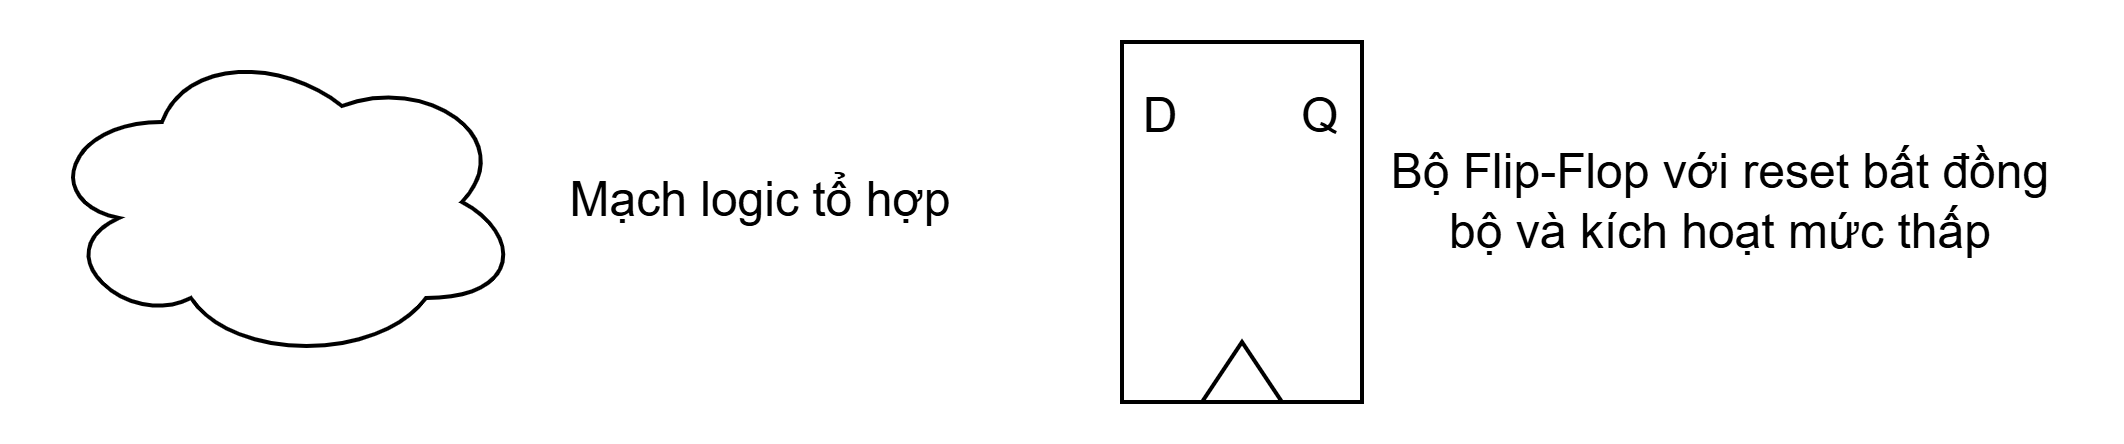
\includegraphics[width=1\linewidth]{figures/commonSymbol.png}
    \caption{Định nghĩa các ký hiệu được sử dụng khi mô tả kiến trúc RTL}
    \label{fig:commonSymbol}
\end{figure}
\section{Mô đun MedianProcessing}
\subsection{Mô đun LineBuffer}
Nguyên lý hoạt động của mô đun LineBuffer là khi có dữ liệu đầu vào, dữ liệu sẽ được ghi vào một vùng nhớ cụ thể, sau khi đạt đến một thời gian hoặc điều kiện đặt ra, dữ liệu từ vùng nhớ đã được ghi sẽ được đọc ra và thứ tự đầu ra sẽ theo nguyên lý FIFO (First In First Out, dữ liệu ghi đầu trước sẽ được đọc ra trước. Hình \ref{fig:lineBuffArchitecture} mô tả kiến trúc RTL của mô đun LineBuffer và hình \ref{fig:lineBufferTrans} mô tả sơ đồ chuyển trạng thái của bộ \textit{controller} cho mô đun này. Có thể mô tả ngắn gọn cách thức hoạt động của mô đun theo mô tả sau: Dữ liệu sẽ được đệm vào bộ nhớ, sau khi dữ liệu ở hàng đầu tiên được đệm (tức là lần đầu tiên bộ nhớ đầy) thì lúc này sẽ có tín hiệu cho phép dữ liệu ra, và quá trình này sẽ kết thúc khi toàn bộ dữ liệu đầu vào được đệm đến đầu ra. 


\textit{Số lượng chu kỳ từ lúc có dữ liệu vào đến khi có dữ liệu đầu ra: } \textbf{DEPTH}


\textit{Số lượng chu kỳ từ lúc có dữ liệu vào đến khi có dữ liệu đầu ra của mô đun Buffer6Rows: } \textbf{3 * DEPTH}


\begin{figure}[!ht]
    \centering
    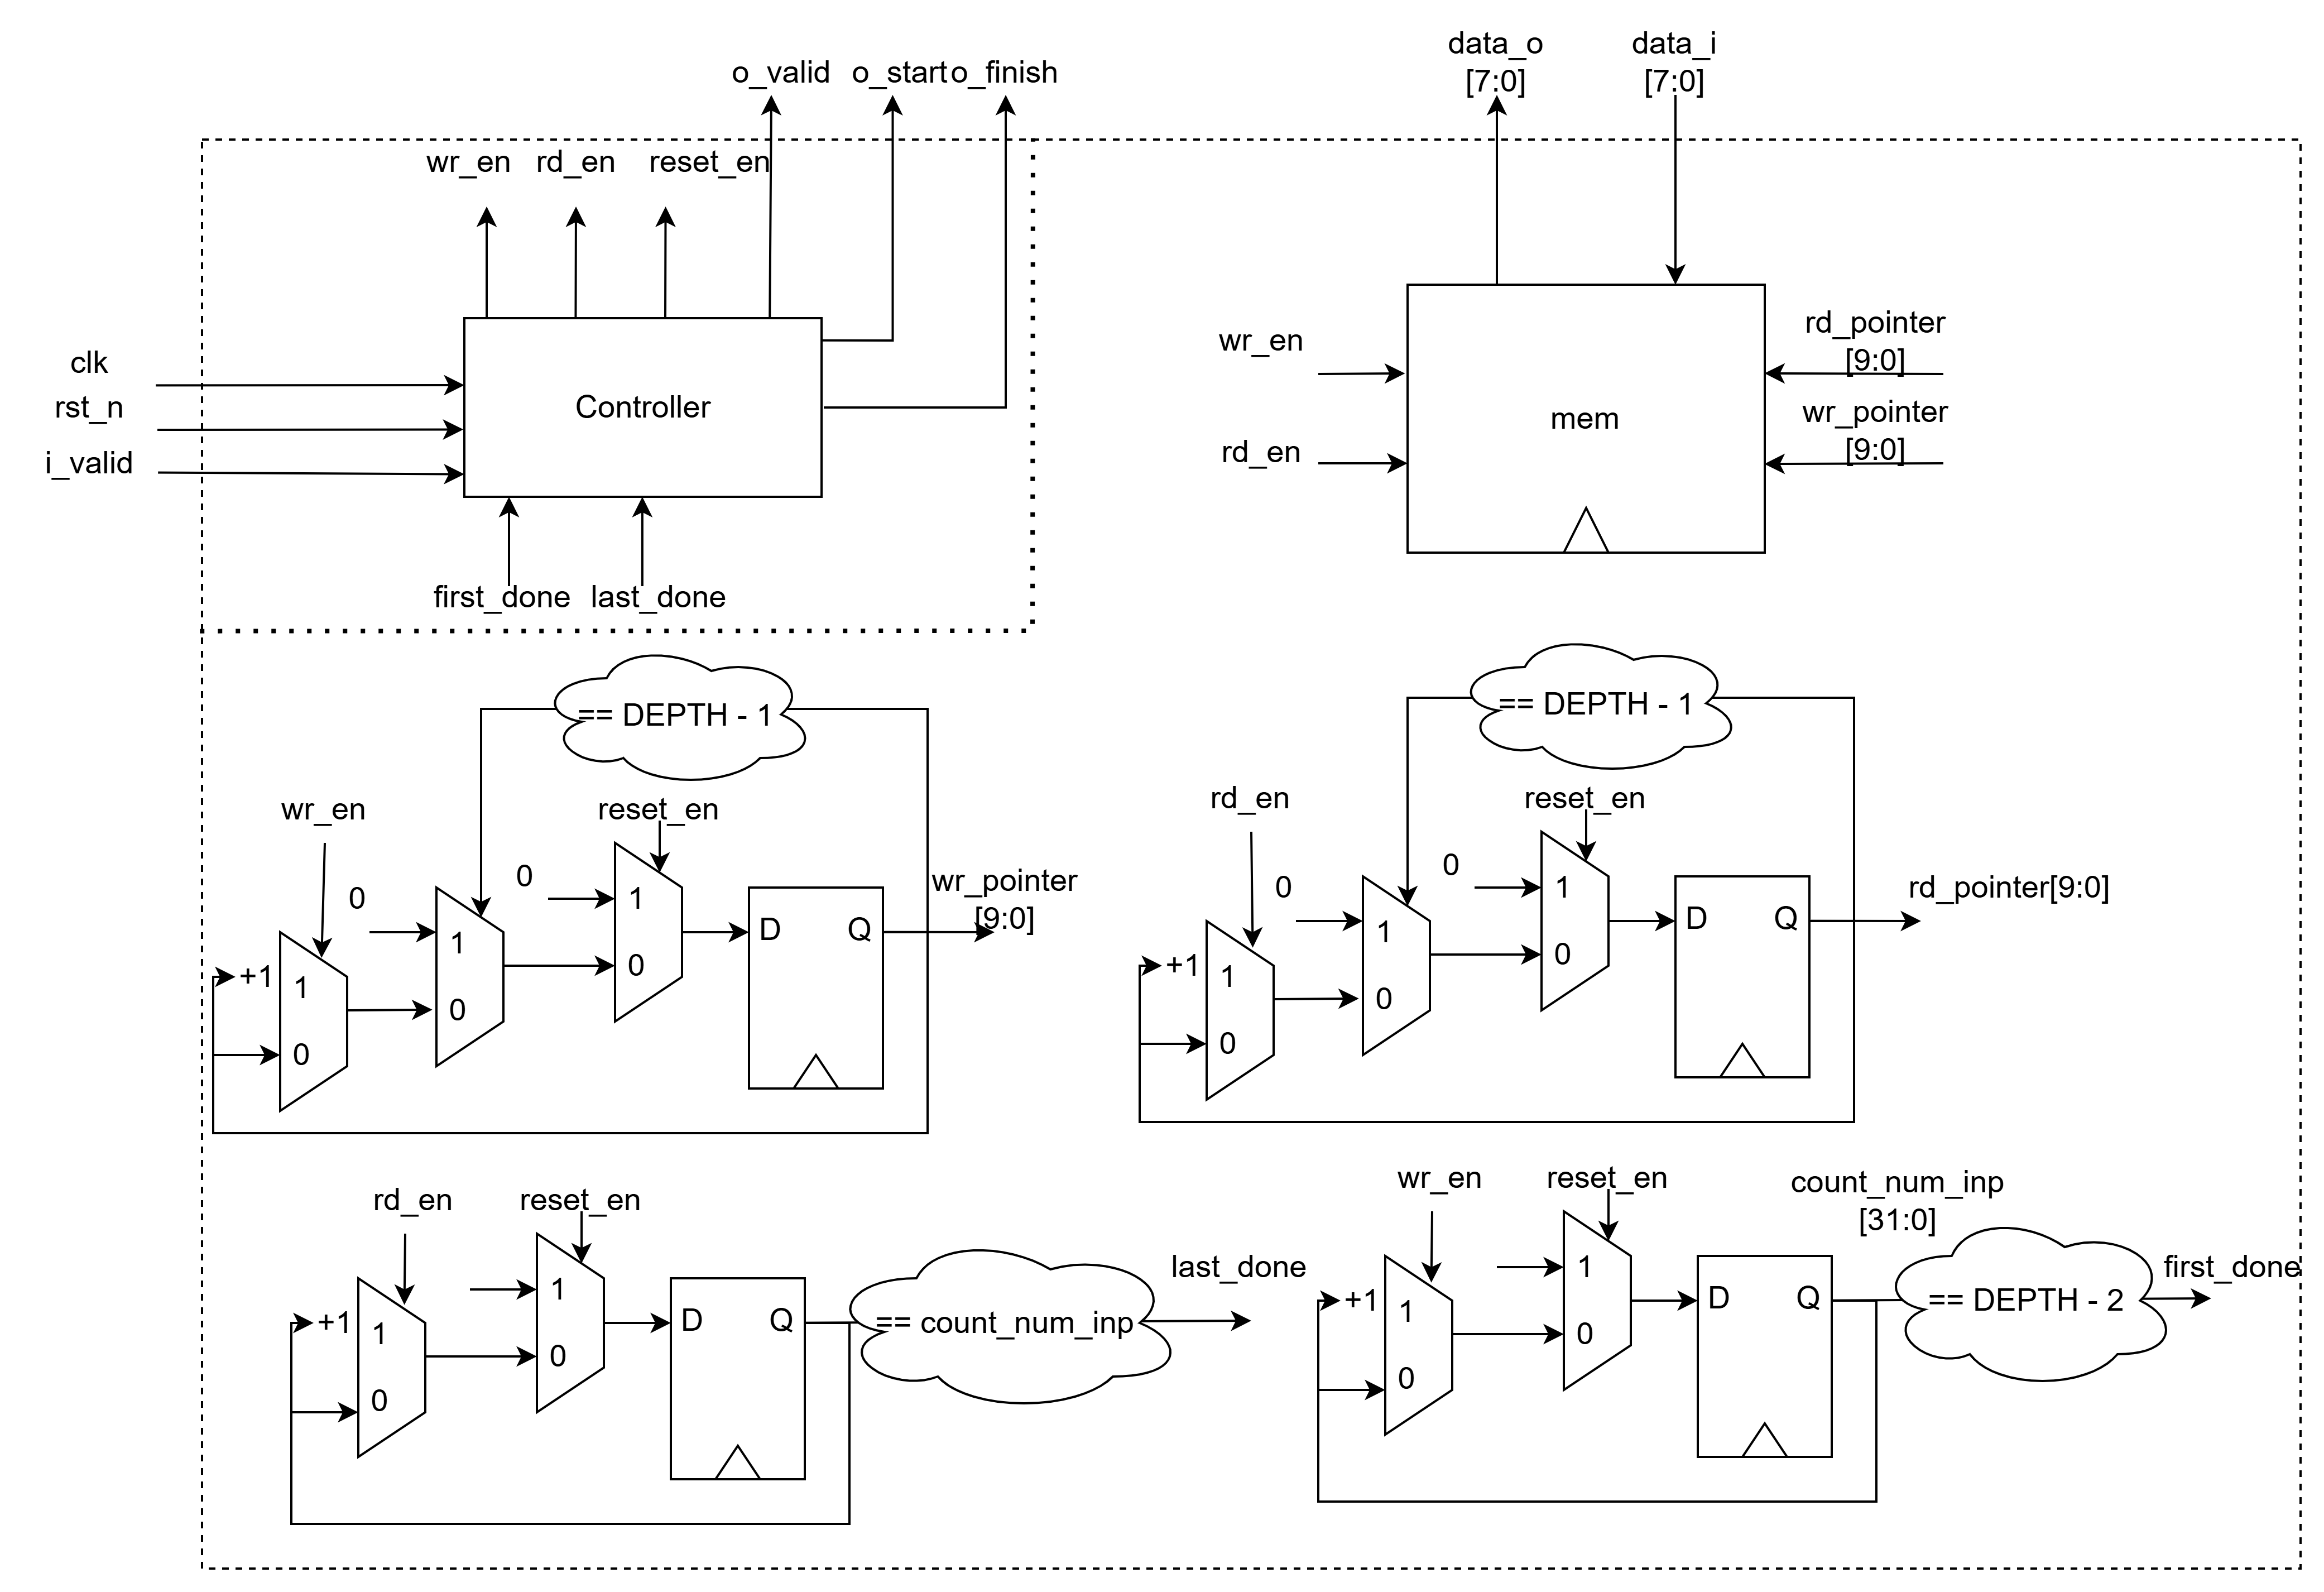
\includegraphics[width=\linewidth]{figures/lineBuffArchitecture.png}
    \caption{Mô tả RTL của mô đun LineBuffer}
    \label{fig:lineBuffArchitecture}
\end{figure}


\begin{figure}[!ht]
    \centering
    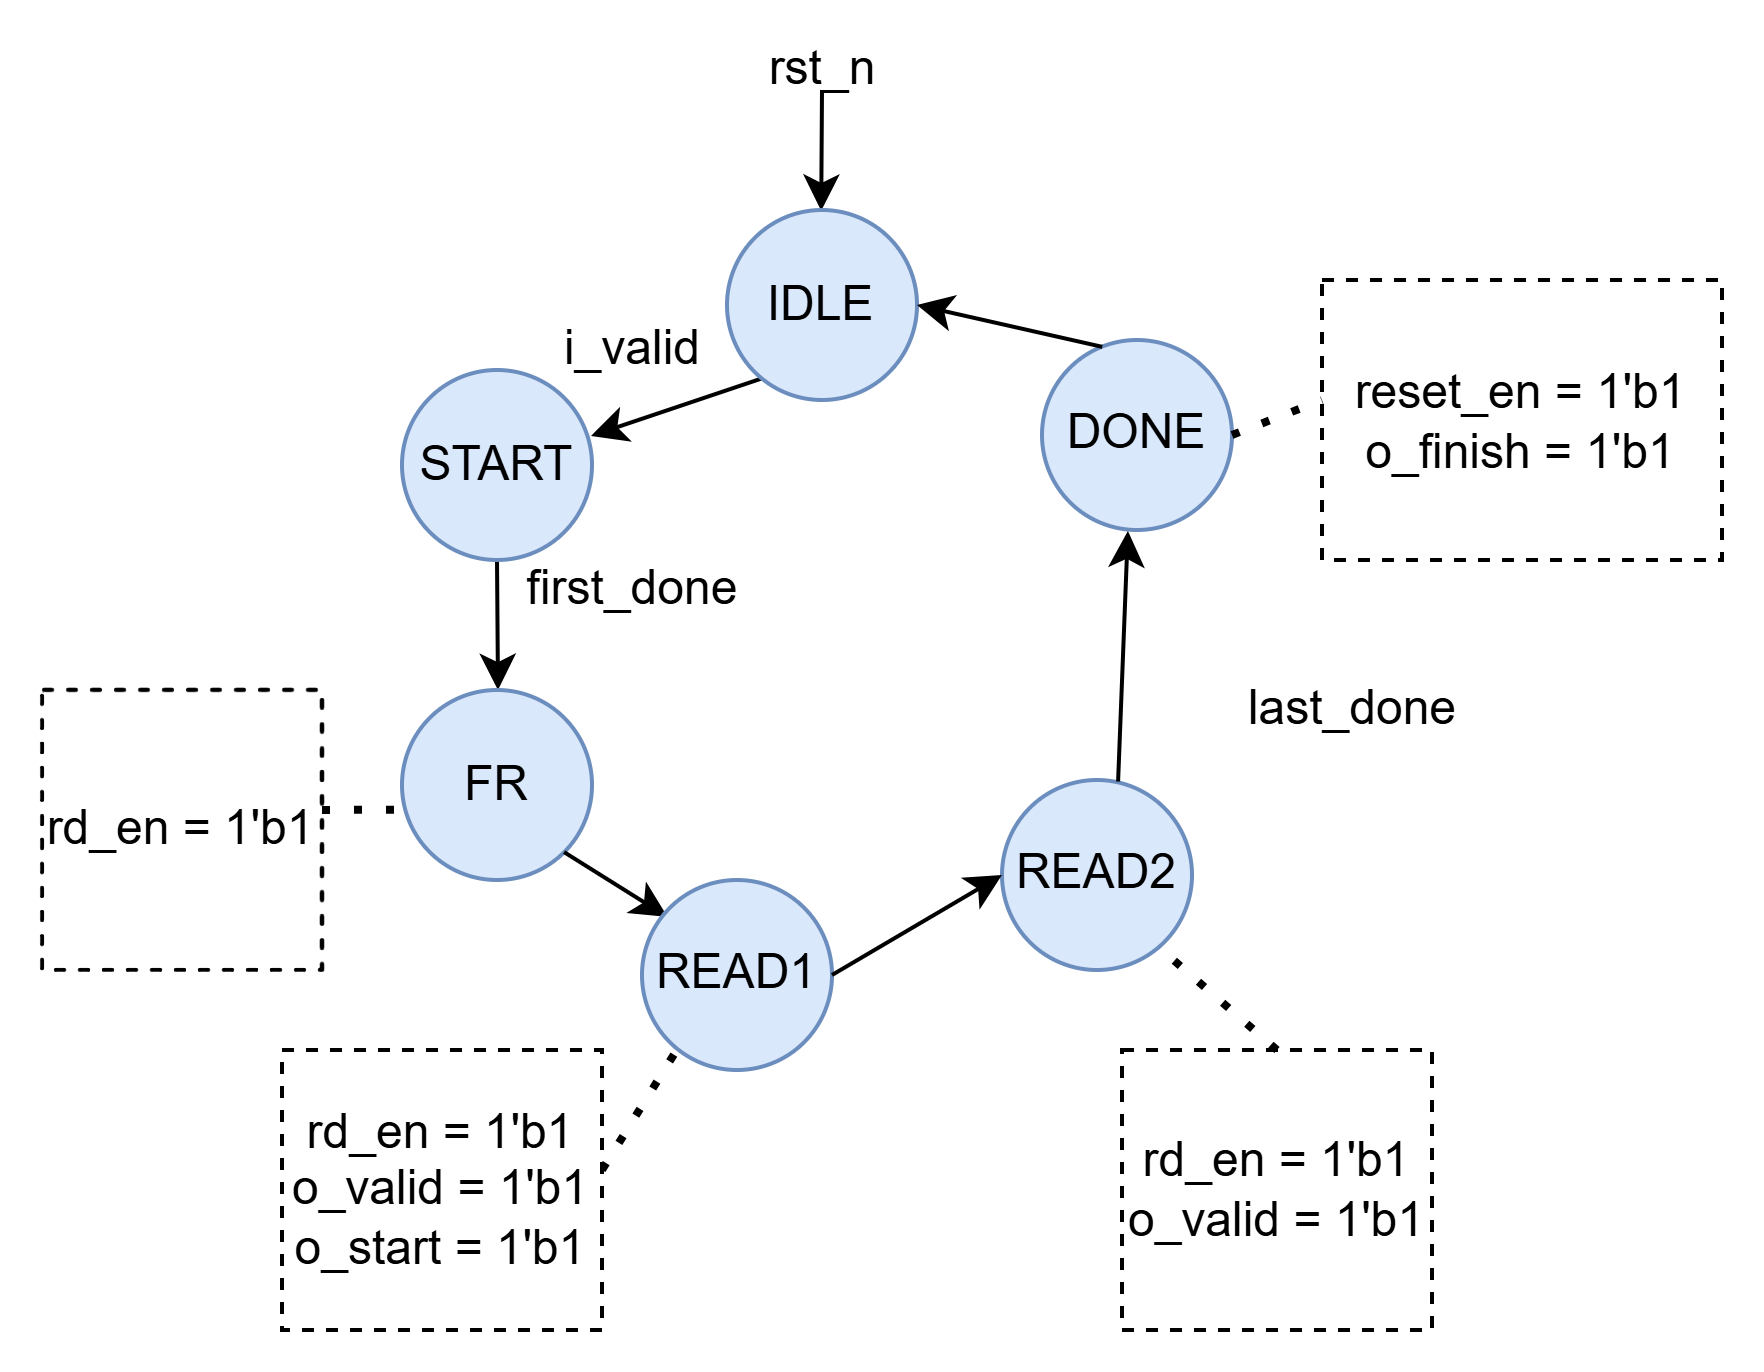
\includegraphics[width=0.8\linewidth]{figures/lineBufferTrans.png}
    \caption{Sơ đồ chuyển trạng thái của mô đun LineBuffer}
    \label{fig:lineBufferTrans}
\end{figure}


\subsection{Mô đun ZeroPadding}
Mô đun ZeroPadding sẽ được thiết kế riêng biệt cho 3 loại cửa sổ là 3x3, 5x5 và 7x7, tuy nhiên chúng đều tồn tại chung một bộ điều khiển được hoạt động theo mô tả ở hình \ref{fig:zeroPaddingTrans}. Sẽ có 4 trạng thái tương ứng là IDLE, DATA, DONE VÀ DONE. Trạng thái \textbf{START} có tác dụng đợi khi dữ liệu được đệm trong mô đun ZeroPadding đủ đáp ứng cho đầu ra của cửa sổ, ví dụ với cửa sổ 3x3 thì sẽ cần đệm thêm 1 số 0 khi ở rìa, thì lúc này trong mô đun phải tồn tại đủ 2 dữ liệu điểm ảnh, như vậy thì sau khi đệm sẽ đủ 3 dữ liệu đầu ra ở 1 hàng hoặc 1 cột. Trạng thái \textbf{DATA} có tác dụng cho phép ghi dữ liệu đầu ra.  

\begin{figure}[!ht]
    \centering
    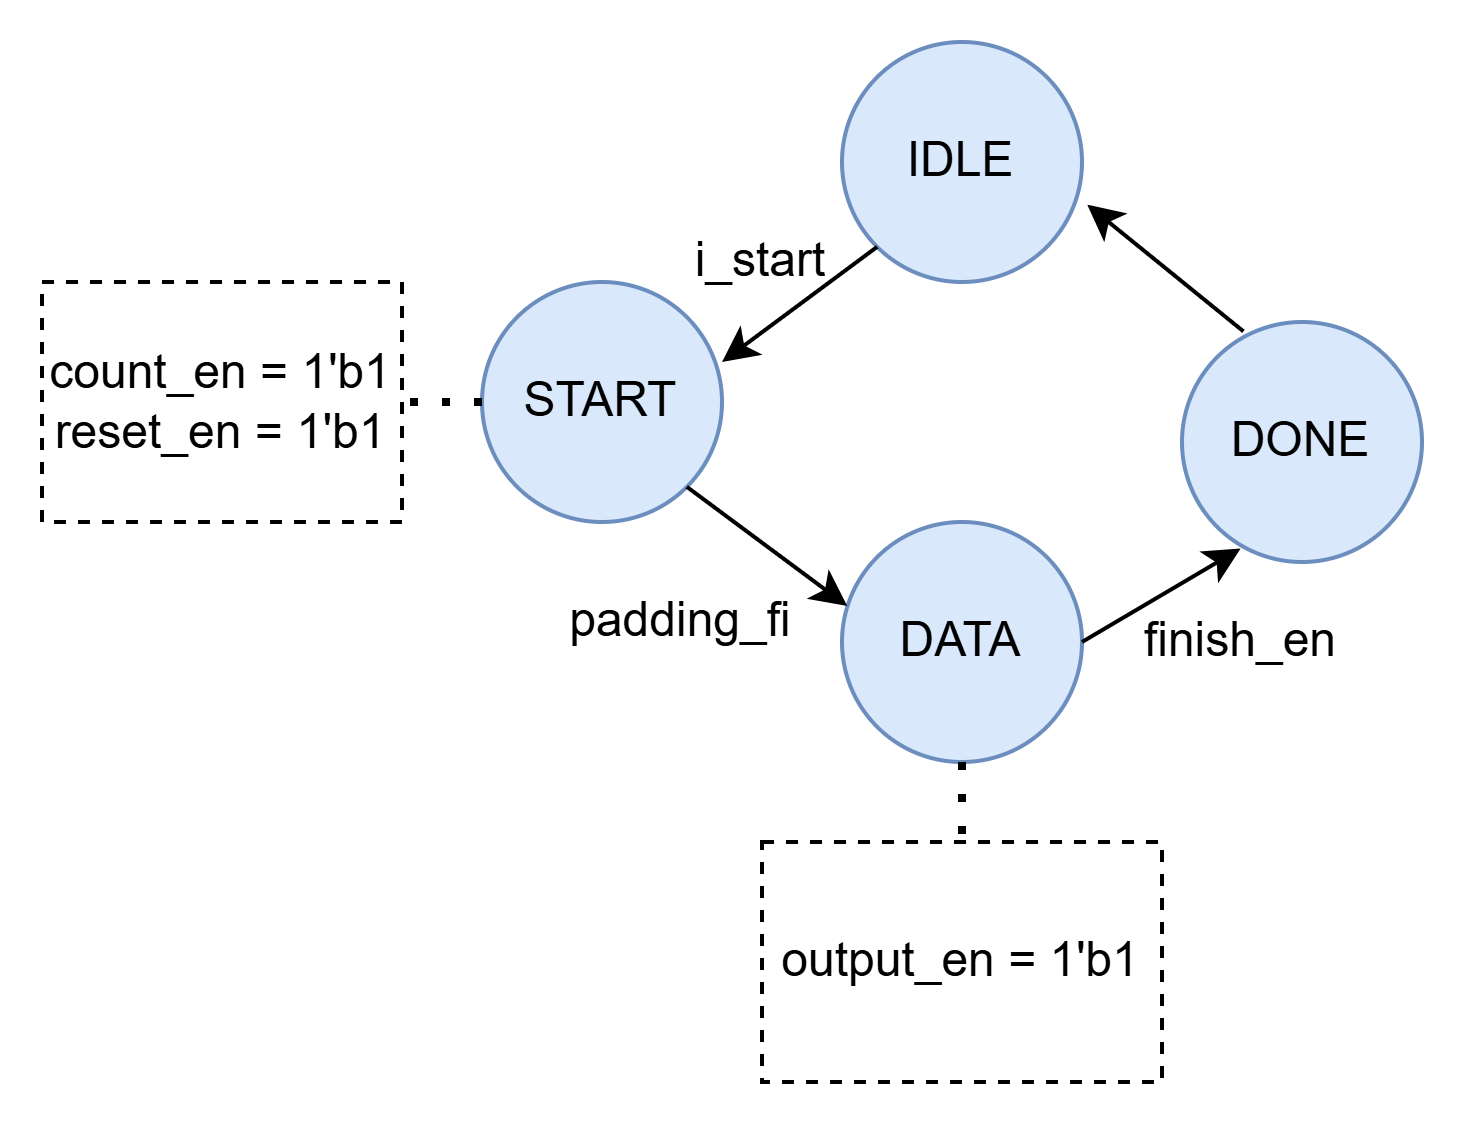
\includegraphics[width=0.7\linewidth]{figures/zeroPaddingTrans.png}
    \caption{Sơ đồ chuyển trạng thái của mô đun ZeroPadding}
    \label{fig:zeroPaddingTrans}
\end{figure}


\subsubsection{Cửa sổ 3x3}
Hình \ref{fig:zero3x3Architecture1} và \ref{fig:zero3x3Architecture2} mô tả kiến trúc RTL đối với bộ ZeroPadding của cửa sổ 3x3, dữ liệu đầu vào của từng hàng sẽ được đệm qua 3 thanh ghi để tạo ra 3 giá trị ứng với mỗi hàng của cửa sổ đầu ra. Dữ liệu đầu ra sẽ dựa vào các điều kiện như ở hình \ref{fig:zero3x3Architecture2}, chính là các tín hiệu điều khiển bộ mạch ghép kênh (mux) để lựa chọn đầu ra là dữ liệu nào.
\begin{figure}[!ht]
    \centering
    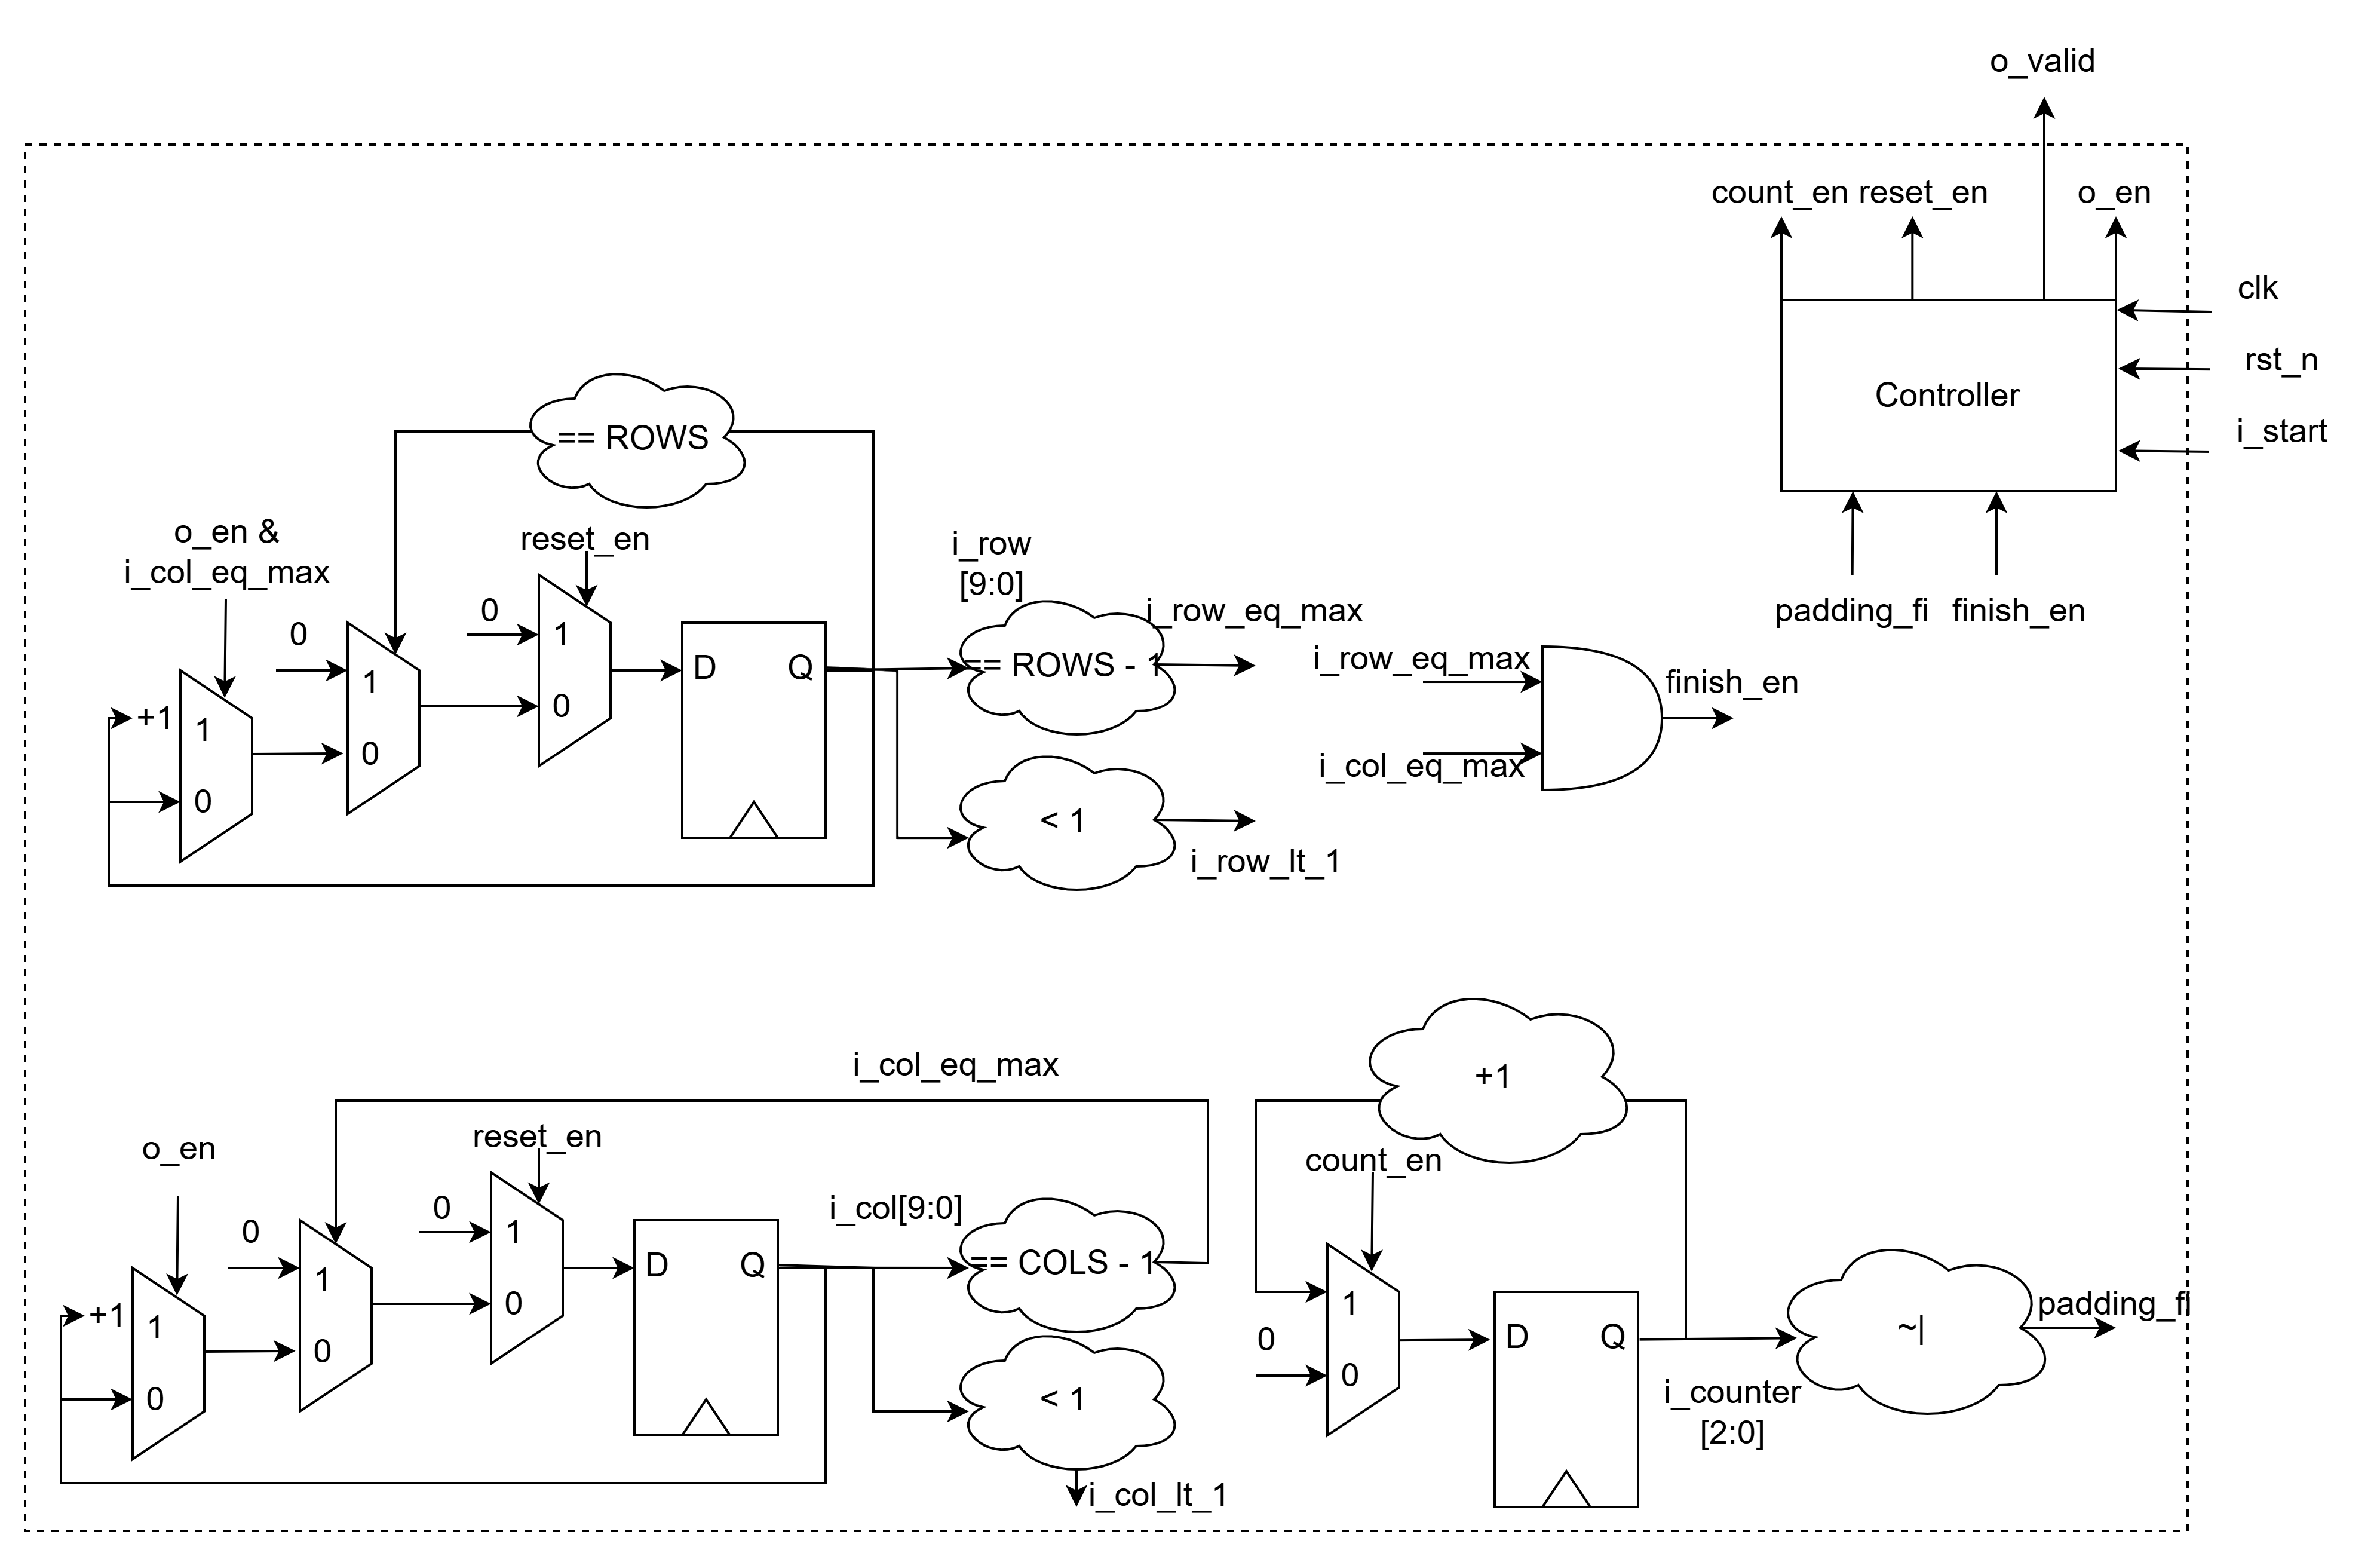
\includegraphics[width=\linewidth]{figures/zero3x3Architecture1.png}
    \caption{Mô tả RTL (1) của mô đun ZeroPadding ứng với cửa sổ 3x3}
    \label{fig:zero3x3Architecture1}
\end{figure}

\begin{figure}[!ht]
    \centering
    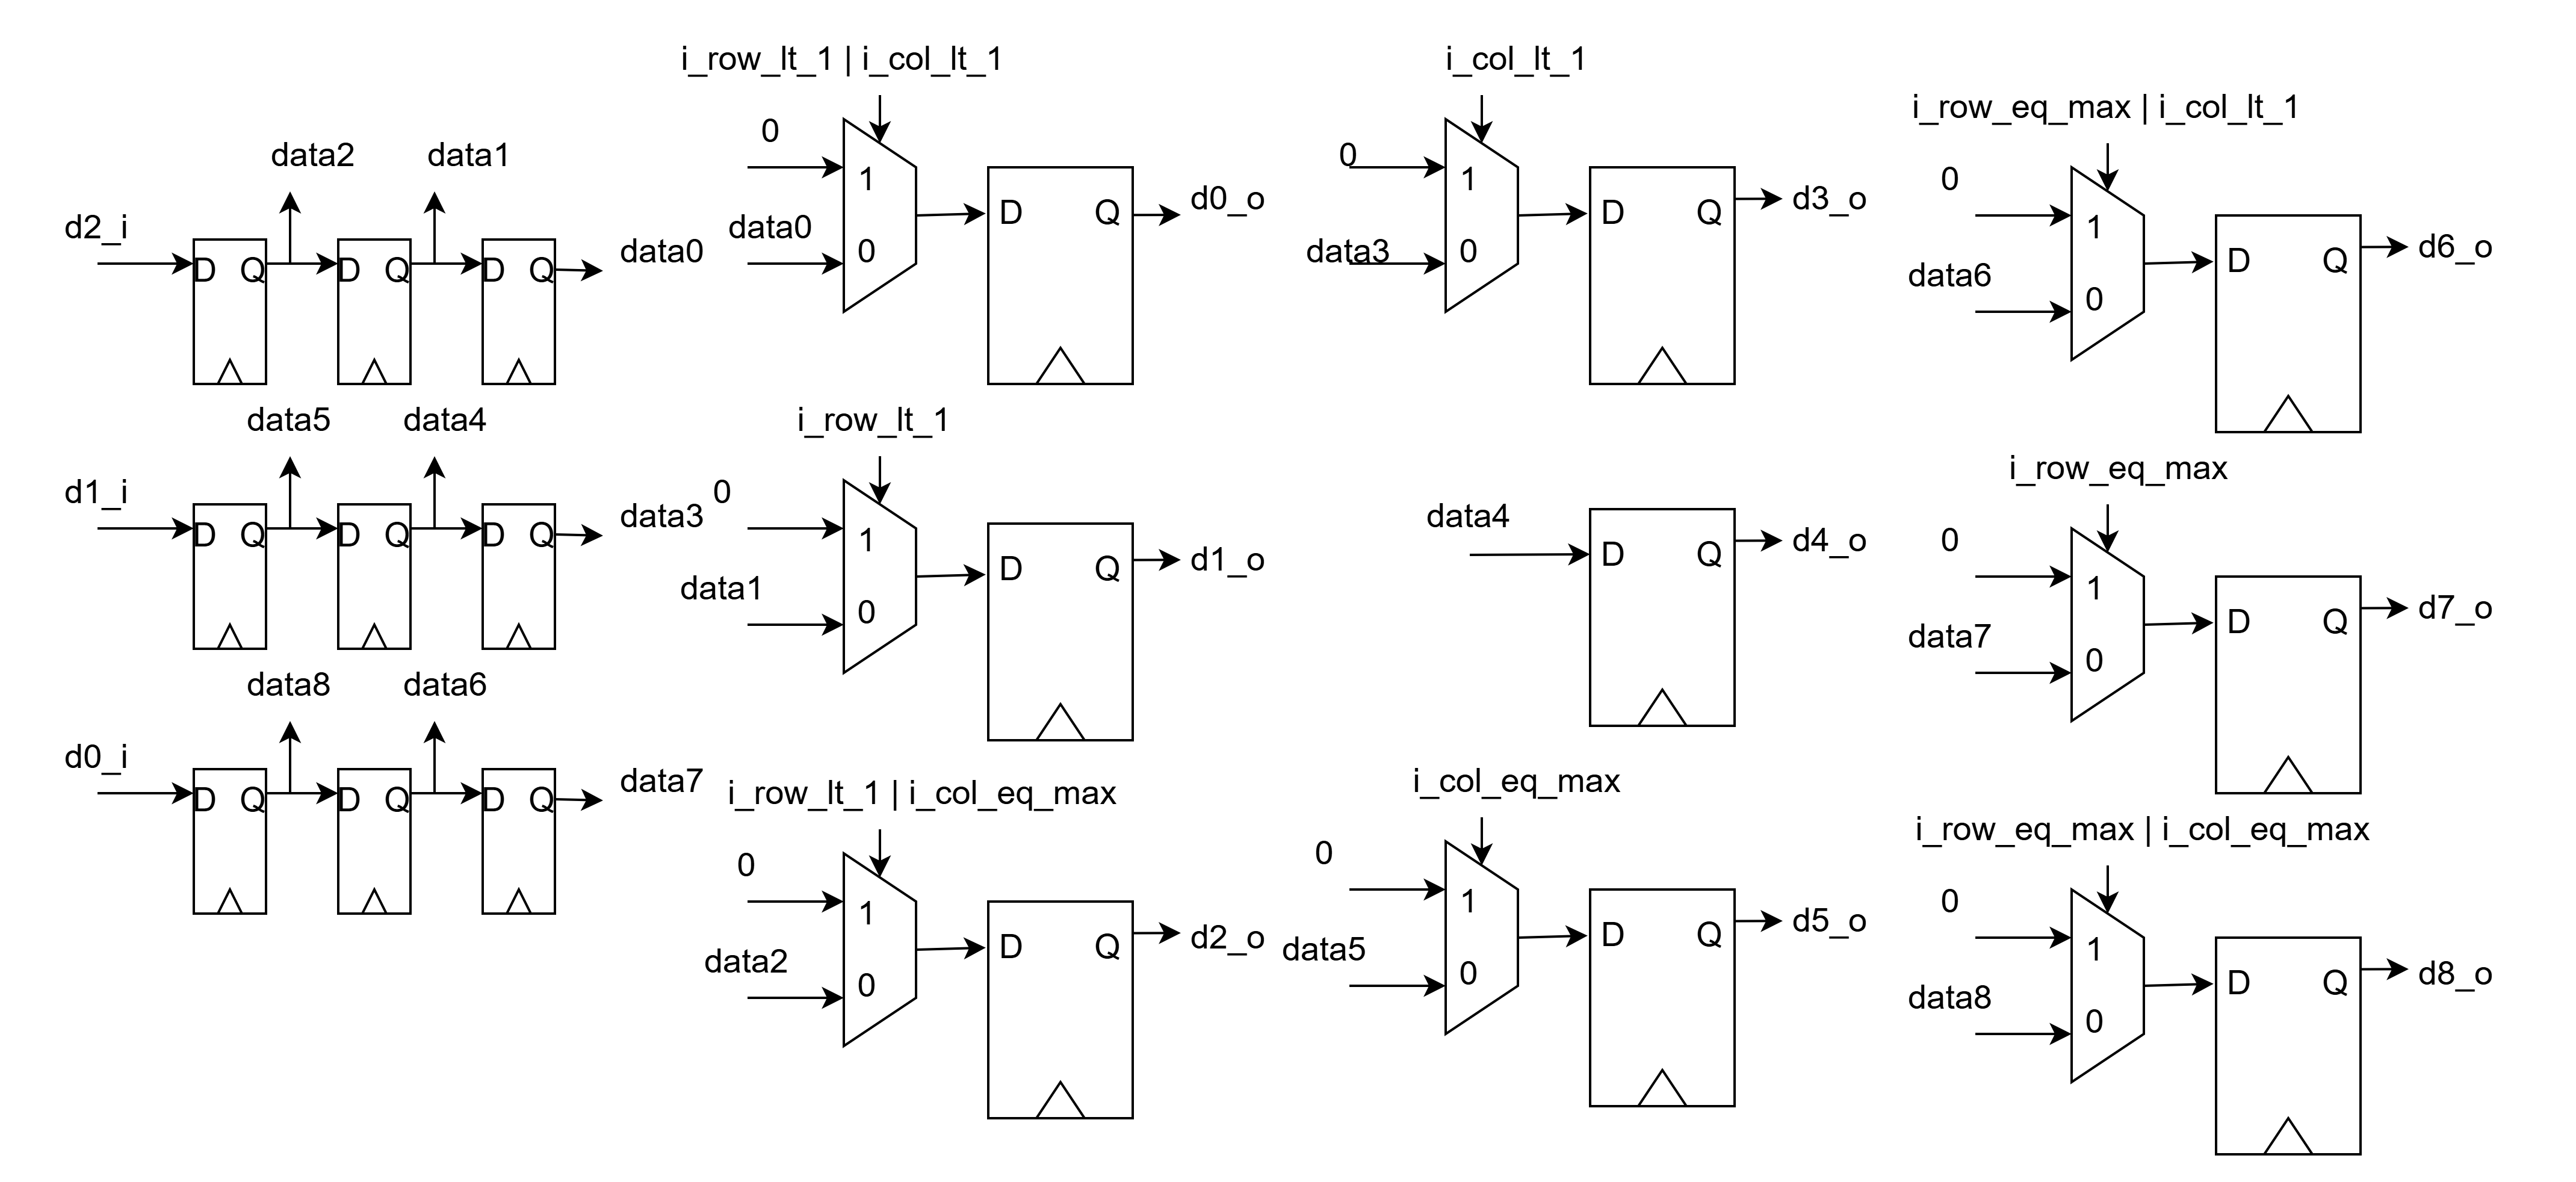
\includegraphics[width=\linewidth]{figures/zero3x3Architecture2.png}
    \caption{Mô tả RTL (2) của mô đun ZeroPadding ứng với cửa sổ 3x3}
    \label{fig:zero3x3Architecture2}
\end{figure}


\textit{
Bởi vì đối với các cửa sổ 5x5 và 7x7, số lượng các đầu vào và điều kiện cho đầu ra là rất nhiều, khó có thể mô tả bằng hình vẽ, do đó sinh viên sẽ đưa ra bảng giá trị tham chiếu và điều kiện cho từng giá trị đầu ra. }
\clearpage
\subsubsection{Cửa sổ 5x5}
Hình \ref{fig:zero5x5Architecture1}, \ref{fig:zero5x5Architecture2} mô tả kiến trúc ở mức RTL cho mô đun ZeroPadding ứng với cửa sổ đầu vào 5x5. Về cơ bản, nguyên lý hoạt động của mô đun này tương tự như đối với cửa sổ 3x3, nhưng có thêm một vài điều kiện thêm cho đầu ra như i\_row\_gt\_row\_3, ... Những điều kiện cho đầu ra đã được mô tả chi tiết trong bảng \ref{tab:conditionForOutputZero5x5}. Cột điều kiện tương ứng với tín hiệu chọn cho bộ mạch ghép kênh, khi điều kiện đúng thì đầu ra sẽ là 0, khi điều kiện sai, dữ liệu đầu ra sẽ ứng với giá trị của giá trị tham chiếu đến.


\begin{figure}[!ht]
    \centering
    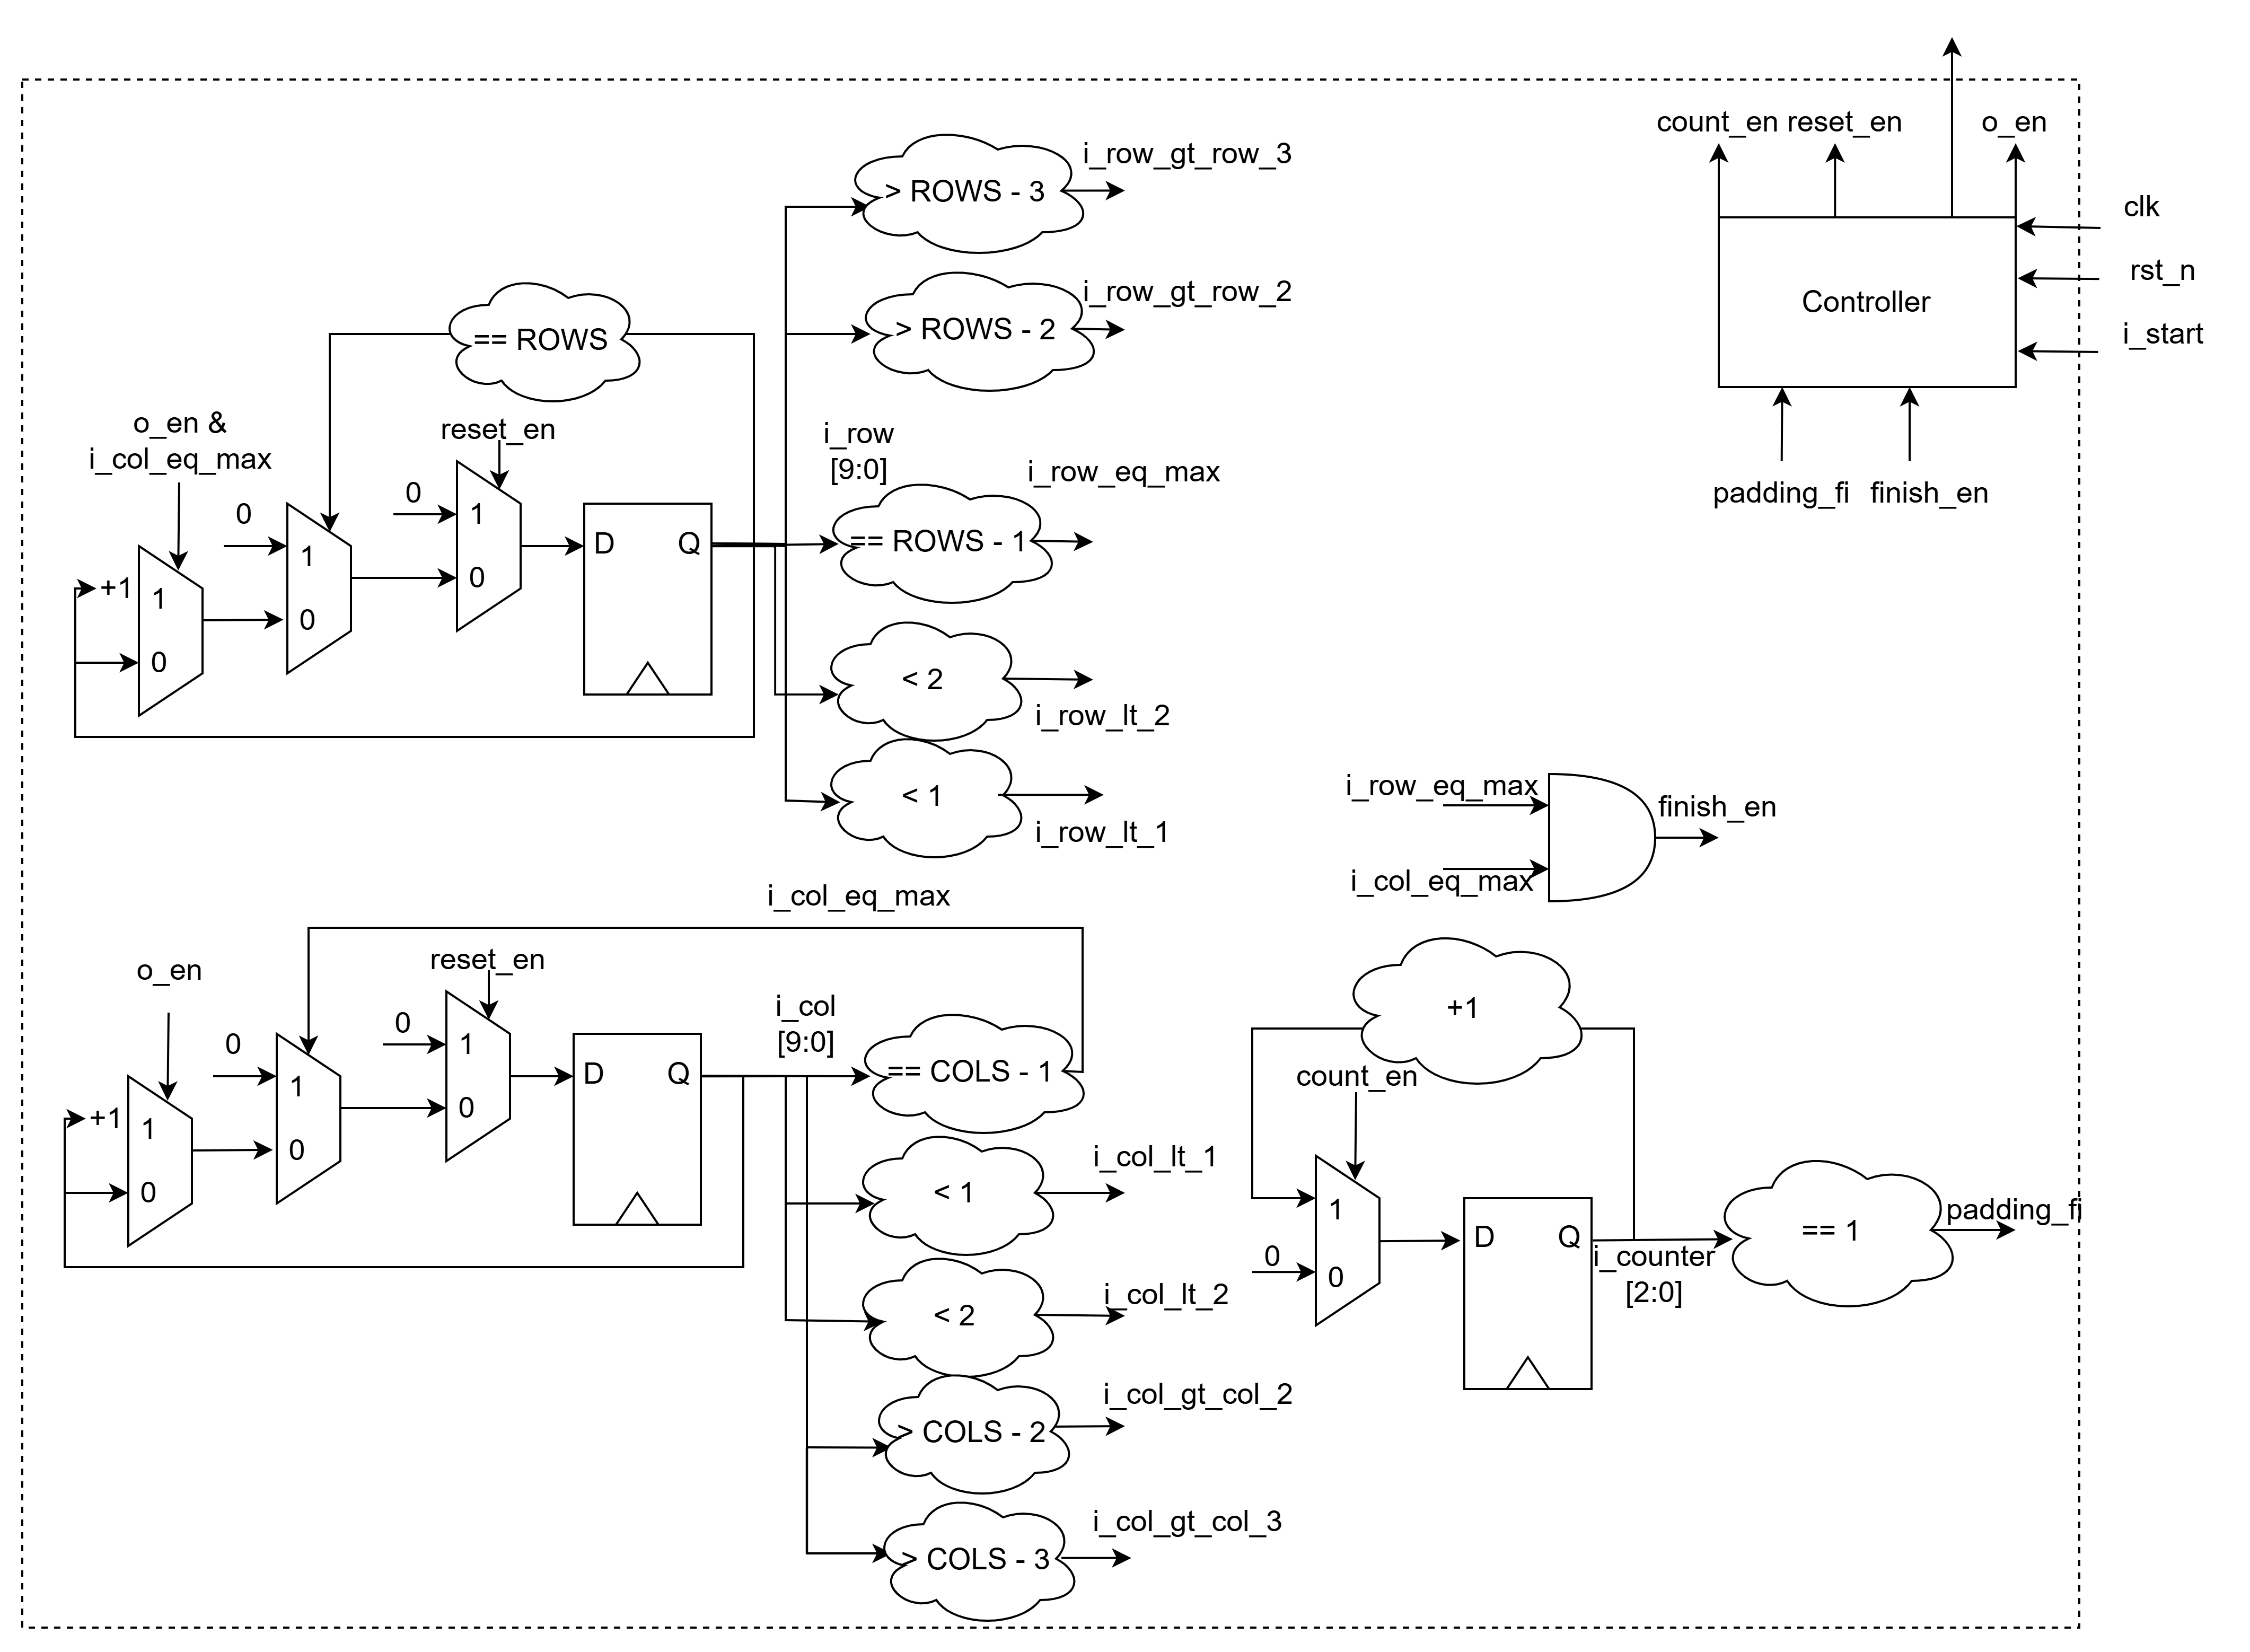
\includegraphics[width=\linewidth]{figures/zero5x5Architecture1.png}
    \caption{Mô tả RTL (1) của mô đun ZeroPadding ứng với cửa sổ 5x5}
    \label{fig:zero5x5Architecture1}
\end{figure}

\begin{figure}[H]
    \centering
    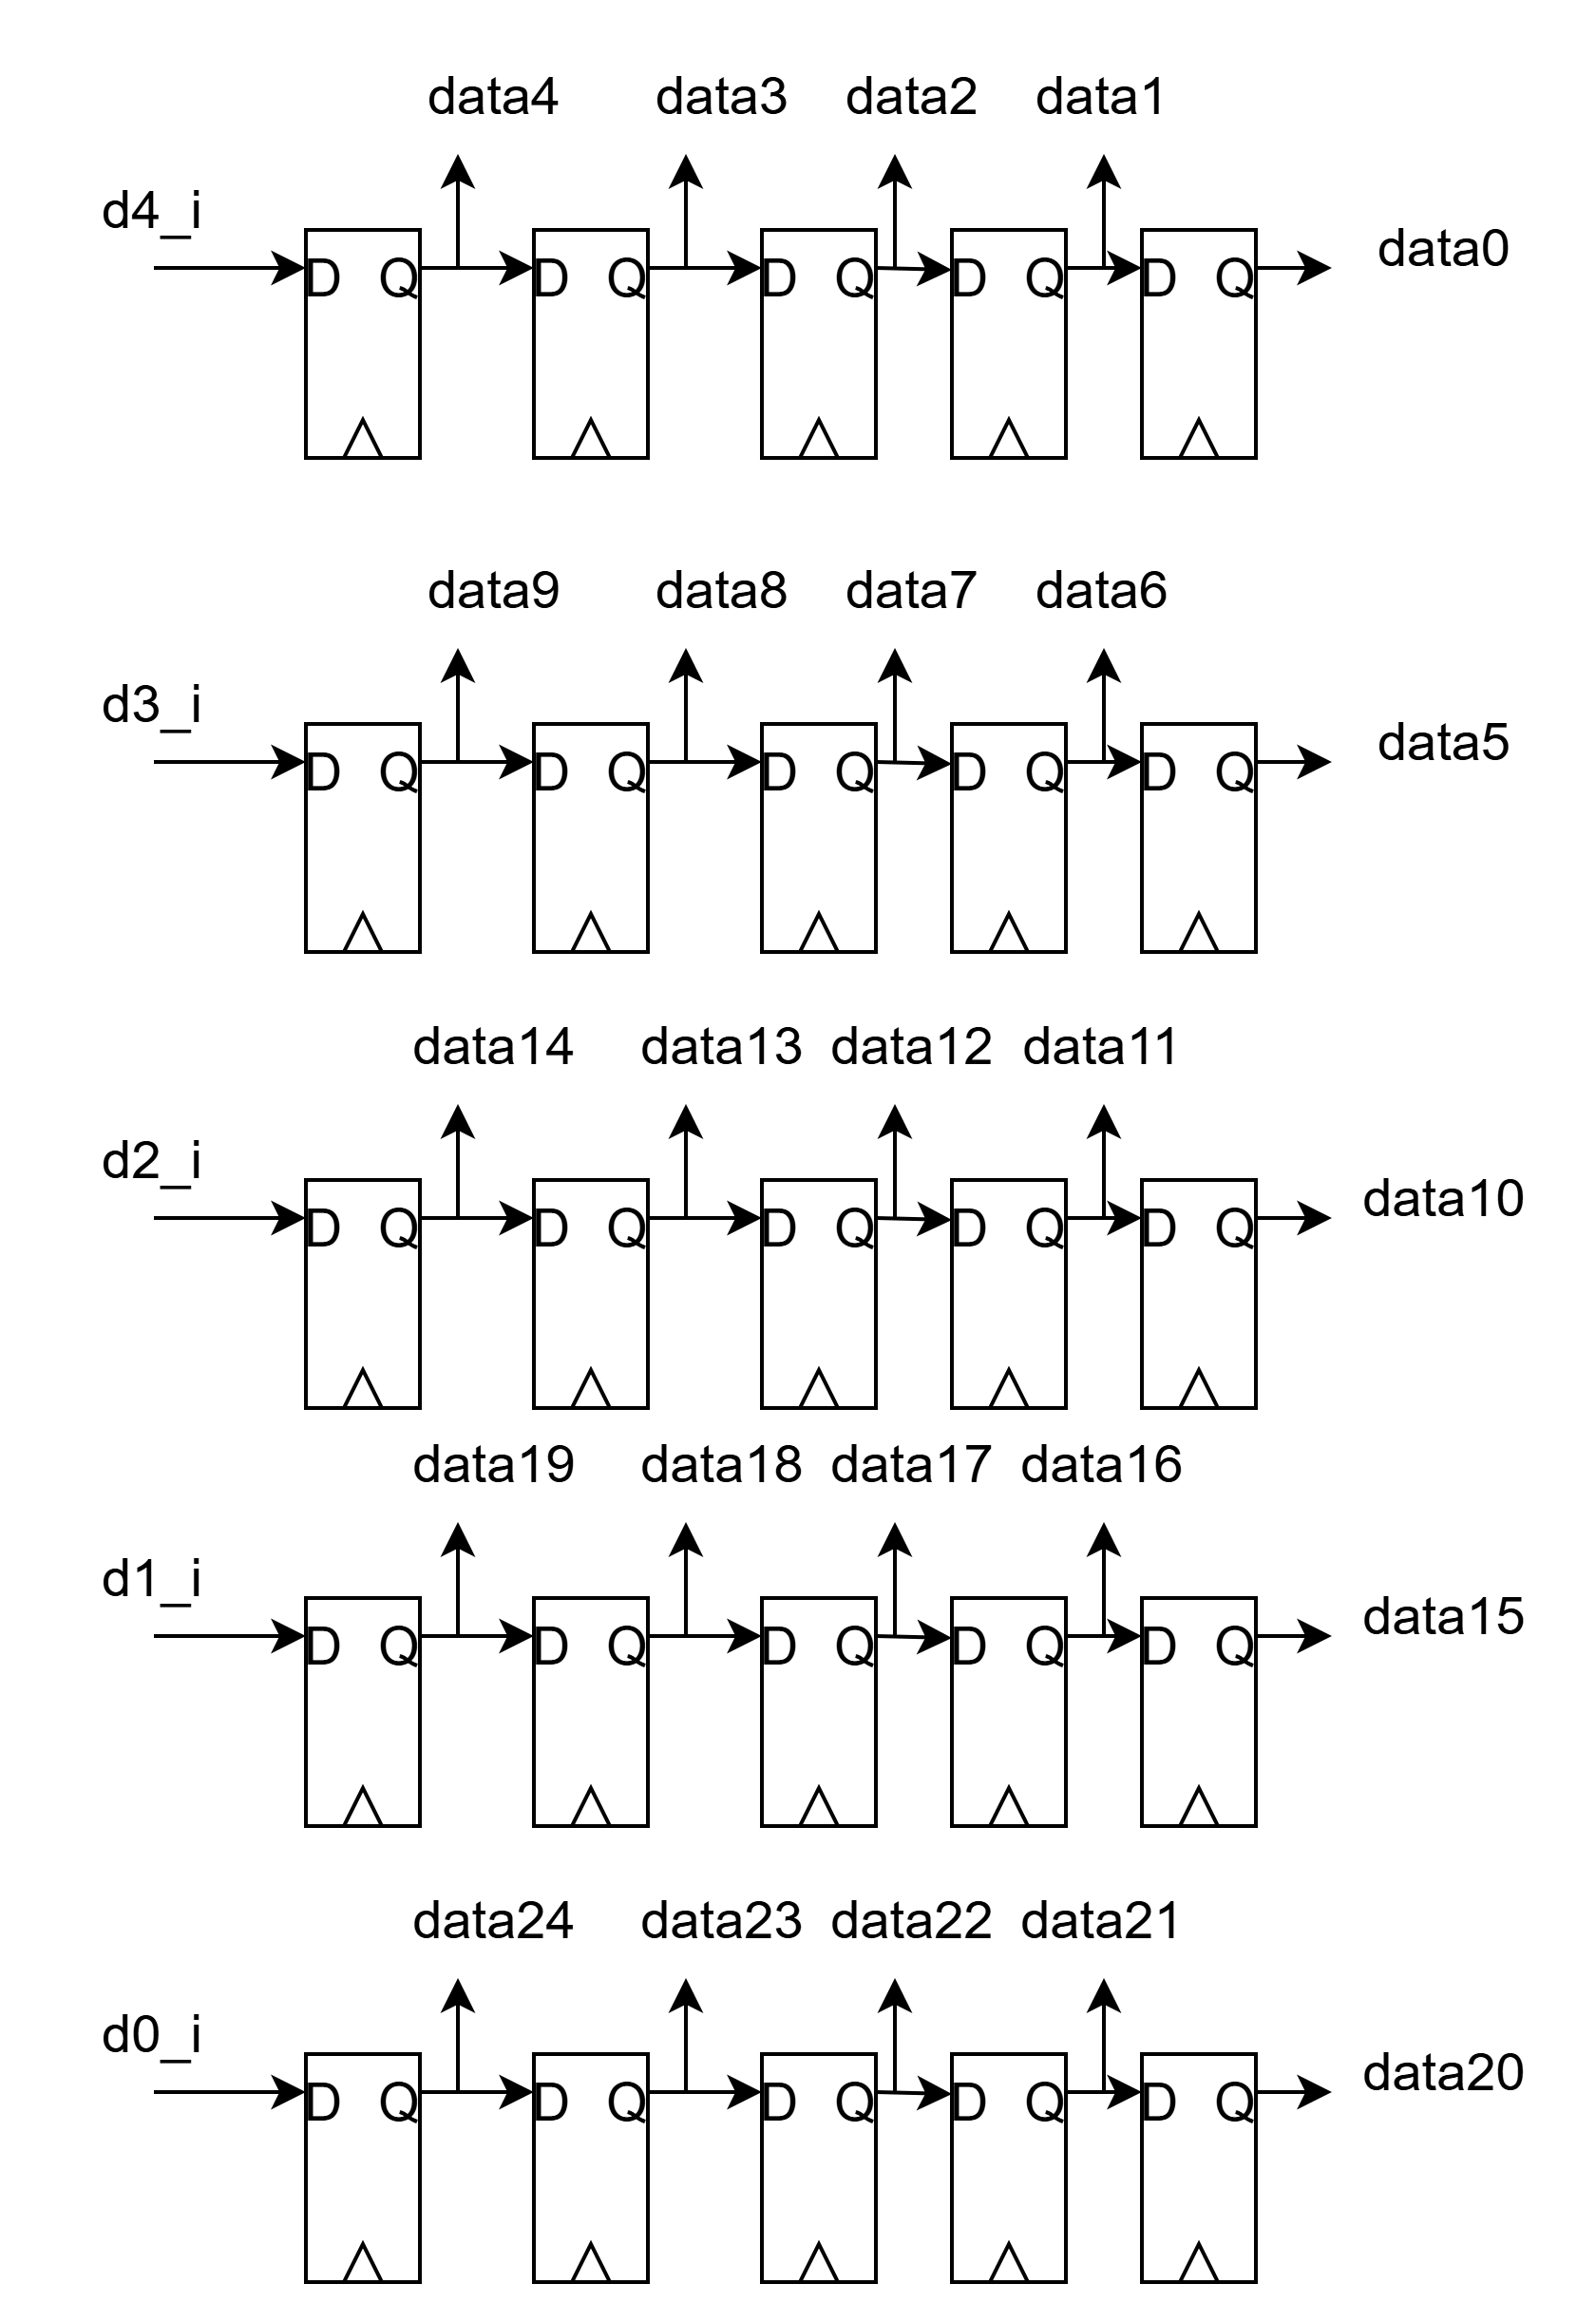
\includegraphics[width=\linewidth]{figures/zero5x5Architecture2.png}
    \caption{Mô tả RTL (2) của mô đun ZeroPadding ứng với cửa sổ 5x5}
    \label{fig:zero5x5Architecture2}
\end{figure}
\begin{table}[H]
    \centering
    \renewcommand{\arraystretch}{1.3}
    \begin{tabular}{|p{2.2cm} p{7cm} p{4cm}|}
        \hline
        \rowcolor{gray!30}
        \textbf{Tên đầu ra} & \textbf{Điều kiện} & \textbf{Giá trị tham chiếu} \\
        \hline
        d0\_o  & i\_row\_lt\_2 $\vert$ i\_col\_lt\_2         & data0  \\ \hline
        d1\_o  & i\_row\_lt\_2 $\vert$ i\_col\_lt\_1         & data1  \\ \hline
        d2\_o  & i\_row\_lt\_2                                & data2  \\ \hline
        d3\_o  & i\_row\_lt\_2 $\vert$ i\_col\_gt\_col\_2     & data3  \\ \hline
        d4\_o  & i\_row\_lt\_2 $\vert$ i\_col\_gt\_col\_3     & data4  \\ \hline
        d5\_o  & i\_row\_lt\_1 $\vert$ i\_col\_lt\_2         & data5  \\ \hline
        d6\_o  & i\_row\_lt\_1 $\vert$ i\_col\_lt\_1         & data6  \\ \hline
        d7\_o  & i\_row\_lt\_1                                & data7  \\ \hline
        d8\_o  & i\_row\_lt\_1 $\vert$ i\_col\_gt\_col\_2     & data8  \\ \hline
        d9\_o  & i\_row\_lt\_1 $\vert$ i\_col\_gt\_col\_3     & data9  \\ \hline
        d10\_o & i\_col\_lt\_2                                & data10 \\ \hline
        d11\_o & i\_col\_lt\_1                                & data11 \\ \hline
        d12\_o & -- (không có điều kiện)                     & data12 \\ \hline
        d13\_o & i\_col\_gt\_col\_2                           & data13 \\ \hline
        d14\_o & i\_col\_gt\_col\_2                           & data14 \\ \hline
      d15\_o & i\_row\_gt\_row\_2 $\vert$ i\_col\_lt\_2     & data15 \\ \hline
      d16\_o & i\_row\_gt\_row\_2 $\vert$ i\_col\_lt\_1     & data16 \\ \hline
      d17\_o & i\_row\_gt\_row\_2                           & data17 \\ \hline
      d18\_o & i\_row\_gt\_row\_2 $\vert$ i\_col\_gt\_col\_2 & data18 \\ \hline
      d19\_o & i\_row\_gt\_row\_2 $\vert$ i\_col\_gt\_col\_3 & data19 \\ \hline
      d20\_o & i\_row\_gt\_row\_3 $\vert$ i\_col\_lt\_2     & data20 \\ \hline
      d21\_o & i\_row\_gt\_row\_3 $\vert$ i\_col\_lt\_1     & data21 \\ \hline
      d22\_o & i\_row\_gt\_row\_3                           & data22 \\ \hline
      d23\_o & i\_row\_gt\_row\_3 $\vert$ i\_col\_gt\_col\_2 & data23 \\ \hline
      d24\_o & i\_row\_gt\_row\_3 $\vert$ i\_col\_gt\_col\_3 & data24 \\ \hline
    \end{tabular}
    \caption{Bảng điều kiện cho dữ liệu đầu ra ứng với cửa sổ 5x5}
    \label{tab:conditionForOutputZero5x5}
\end{table}

\subsubsection{Cửa sổ 7x7}
\begin{figure}[!ht]
    \centering
    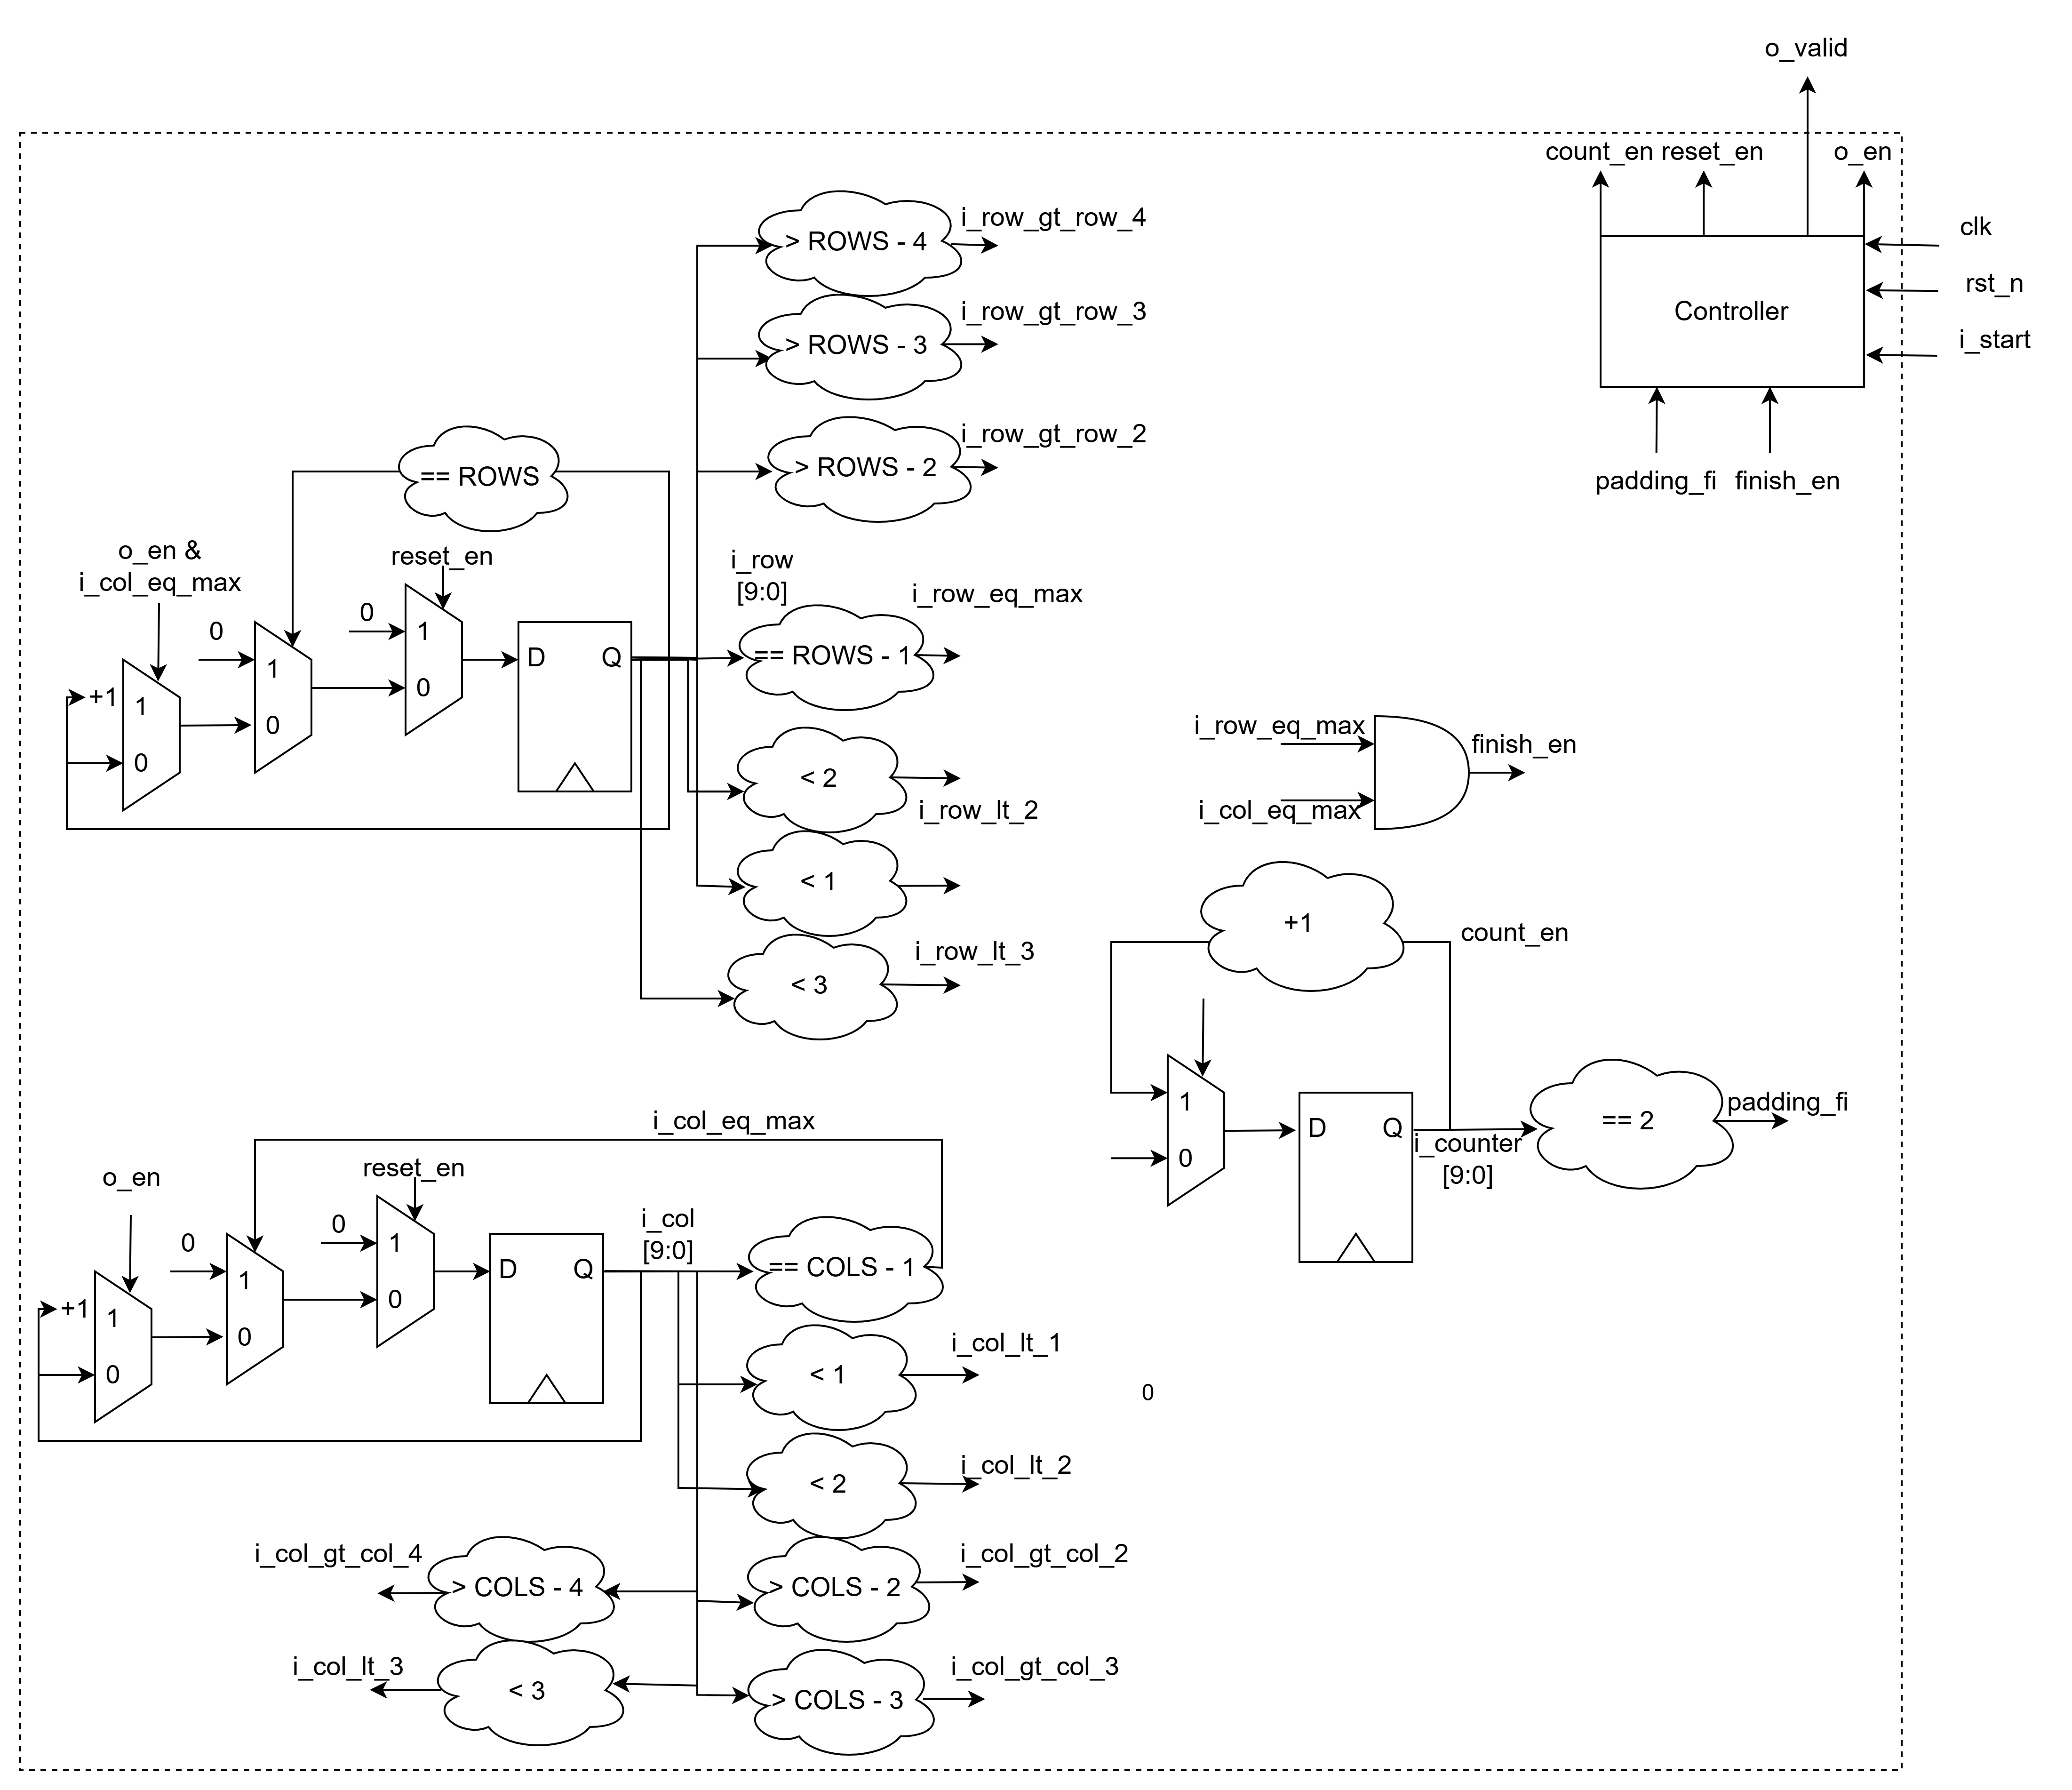
\includegraphics[width=\linewidth]{figures/zero7x7Architecture1.png}
    \caption{Mô tả RTL (1) của mô đun ZeroPadding ứng với cử sổ 7x7}
    \label{fig:zero7x7Architecture1}
\end{figure}
\begin{figure}[H]
	\centering
	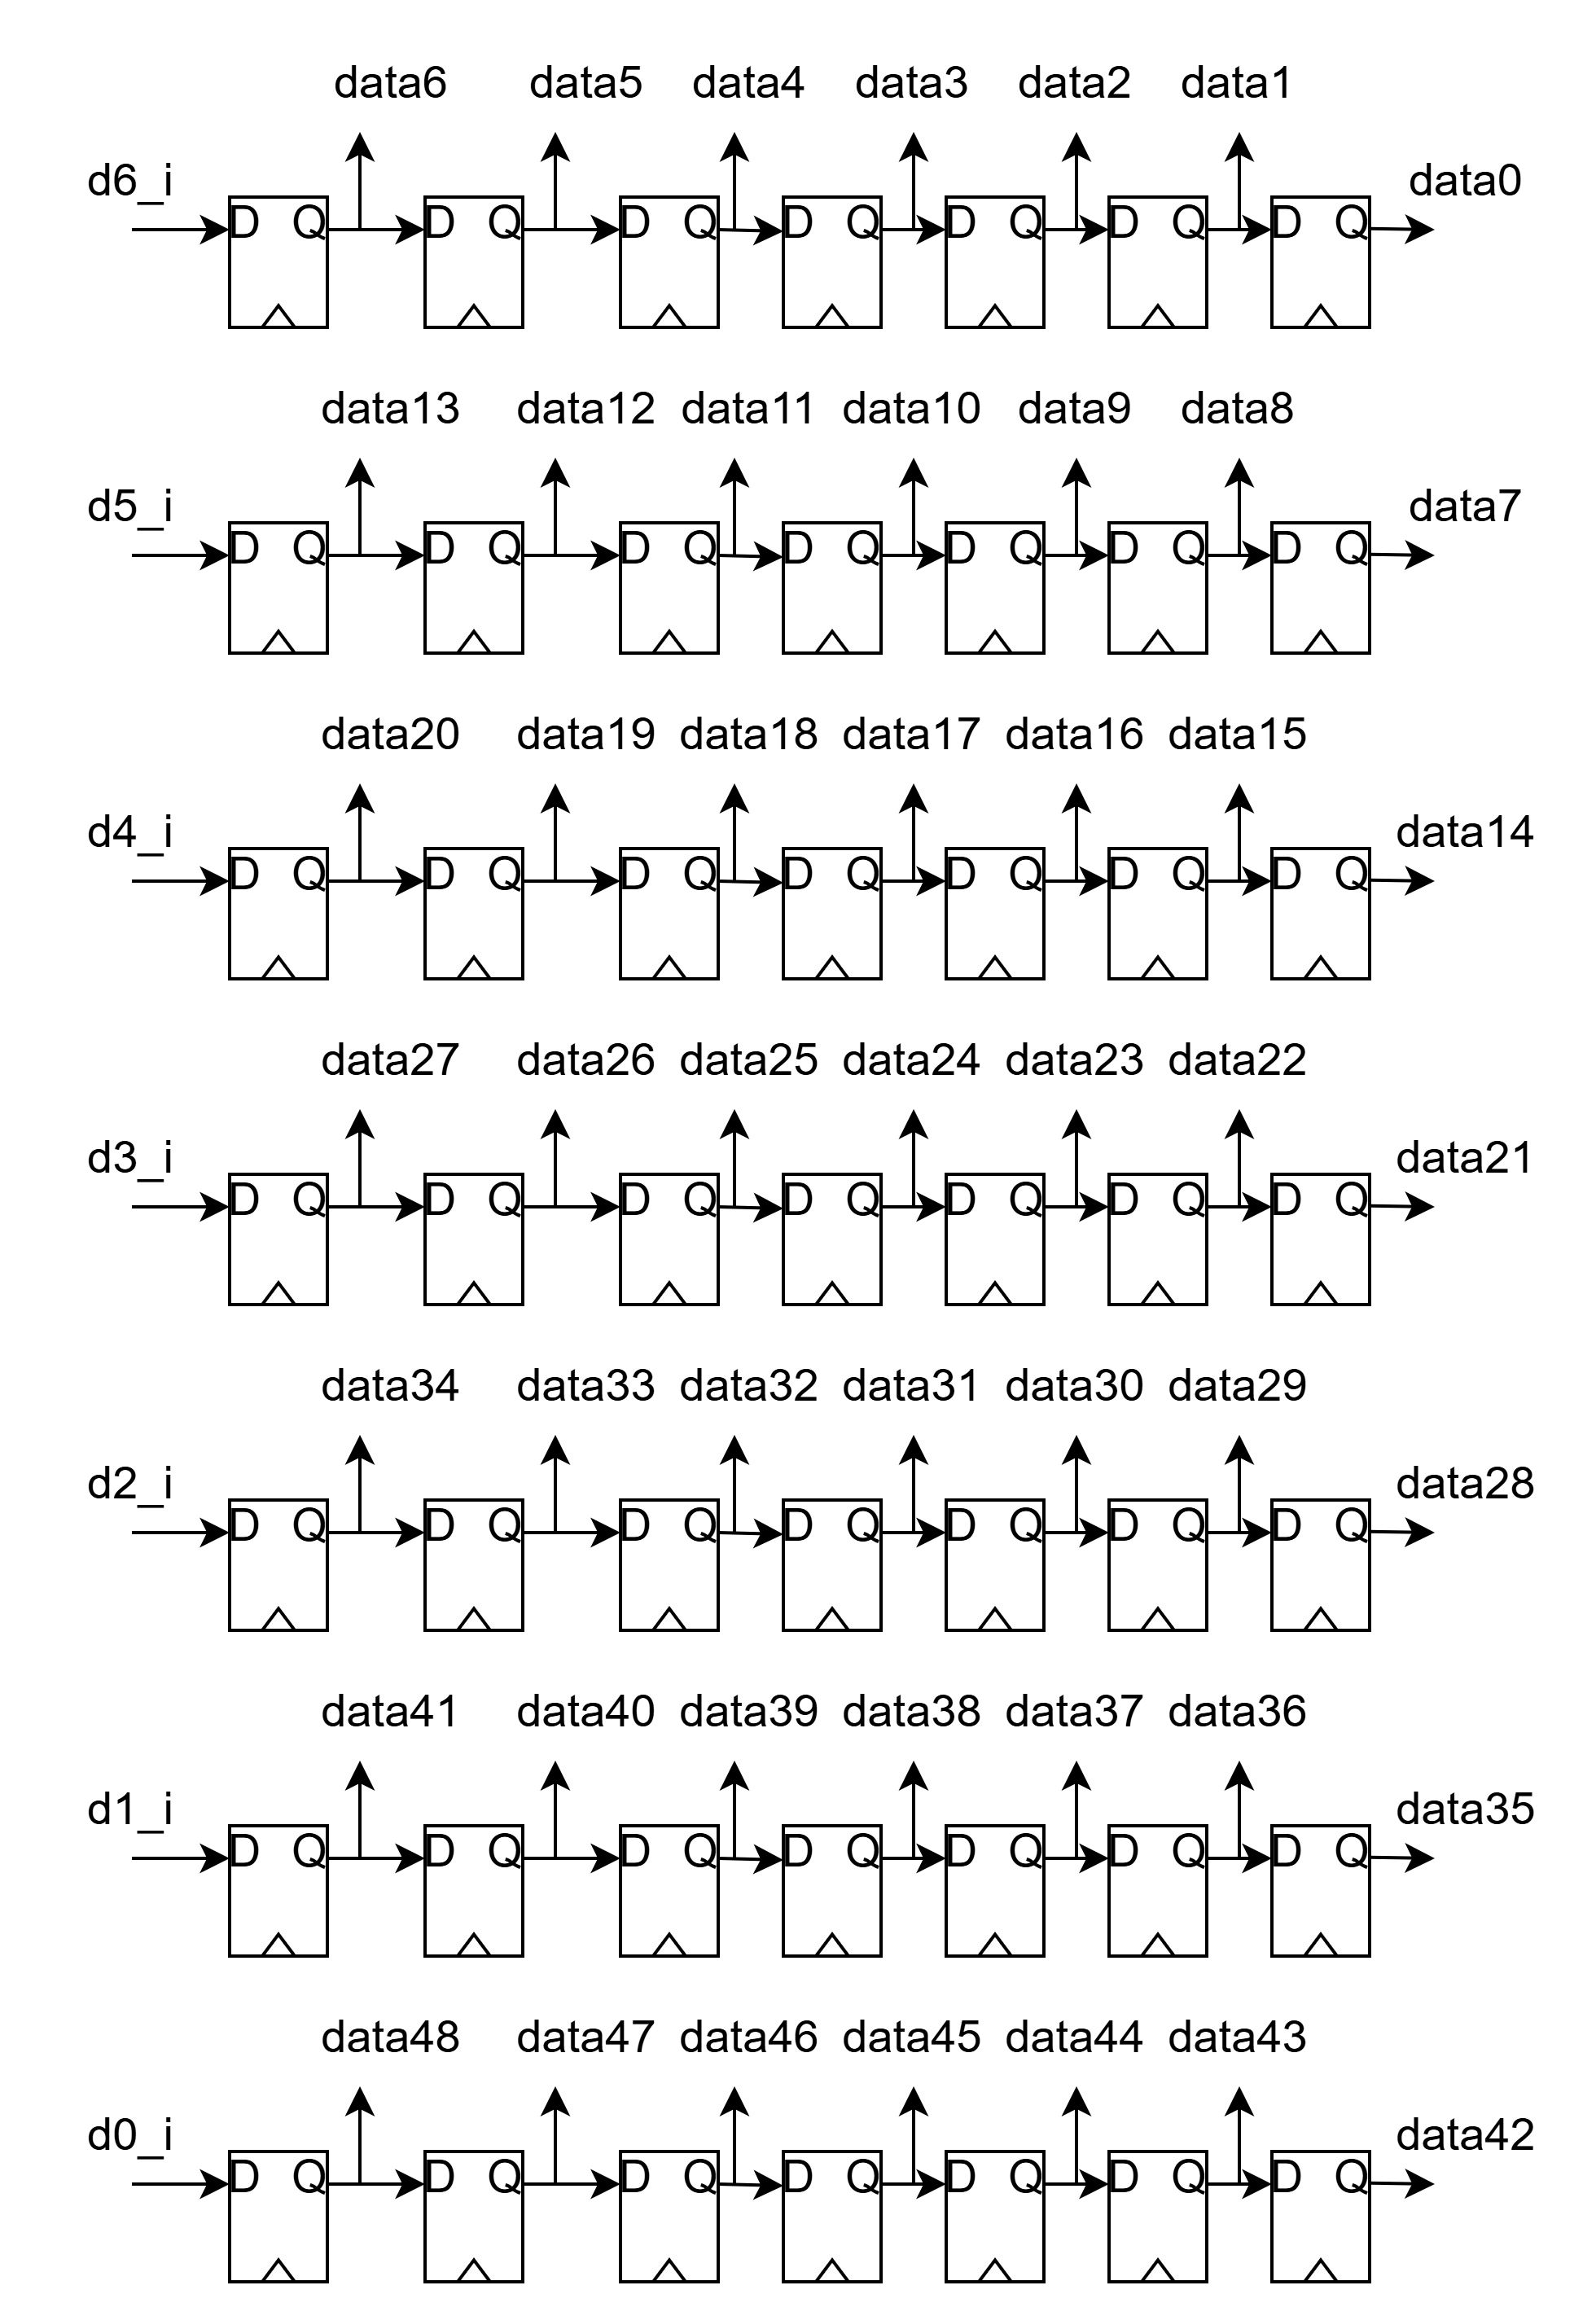
\includegraphics[width=\linewidth]{figures/zero7x7Architecture2.png}
	\caption{Mô tả RTL (2) của mô đun ZeroPadding ứng với cử sổ 7x7}
	\label{fig:zero7x7Architecture2}
\end{figure}


\renewcommand{\arraystretch}{1}
\begin{longtable}{|p{3cm}|p{8cm}|p{4cm}|}
	\hline
	\rowcolor{gray!30}
	\textbf{Tên đầu ra} & \textbf{Điều kiện} & \textbf{Giá trị tham chiếu} \\
	\hline
	\endfirsthead
	
	\hline
	\rowcolor{gray!30}
	\textbf{Tên đầu ra} & \textbf{Điều kiện} & \textbf{Giá trị tham chiếu} \\
	\hline
	\endhead
	d0\_o & i\_row\_lt\_3 $\vert$ i\_col\_lt\_3 & data0 \\
	d1\_o & i\_row\_lt\_3 $\vert$ i\_col\_lt\_2 & data1 \\
	d2\_o & i\_row\_lt\_3 $\vert$ i\_col\_lt\_1 & data2 \\
	d3\_o & i\_row\_lt\_3 & data3 \\
	d4\_o & i\_row\_lt\_3 $\vert$ i\_col\_gt\_col\_2 & data4 \\
	d5\_o & i\_row\_lt\_3 $\vert$ i\_col\_gt\_col\_3 & data5 \\
	d6\_o & i\_row\_lt\_3 $\vert$ i\_col\_gt\_col\_4 & data6 \\
	d7\_o & i\_row\_lt\_2 $\vert$ i\_col\_lt\_3 & data7 \\
	d8\_o & i\_row\_lt\_2 $\vert$ i\_col\_lt\_2 & data8 \\
	d9\_o & i\_row\_lt\_2 $\vert$ i\_col\_lt\_1 & data9 \\
	d10\_o & i\_row\_lt\_2 & data10 \\
	d11\_o & i\_row\_lt\_2 $\vert$ i\_col\_gt\_col\_2 & data11 \\
	d12\_o & i\_row\_lt\_2 $\vert$ i\_col\_gt\_col\_3 & data12 \\
	d13\_o & i\_row\_lt\_2 $\vert$ i\_col\_gt\_col\_4 & data13 \\
	d14\_o & i\_row\_lt\_1 $\vert$ i\_col\_lt\_3 & data14 \\
	d15\_o & i\_row\_lt\_1 $\vert$ i\_col\_lt\_2 & data15 \\
	d16\_o & i\_row\_lt\_1 $\vert$ i\_col\_lt\_1 & data16 \\
	d17\_o & i\_row\_lt\_1 & data17 \\
	d18\_o & i\_row\_lt\_1 $\vert$ i\_col\_gt\_col\_2 & data18 \\
	d19\_o & i\_row\_lt\_1 $\vert$ i\_col\_gt\_col\_3 & data19 \\
	d20\_o & i\_row\_lt\_1 $\vert$ i\_col\_gt\_col\_4 & data20 \\
	d21\_o & i\_col\_lt\_3 & data21 \\
	d22\_o & i\_col\_lt\_2 & data22 \\
	d23\_o & i\_col\_lt\_1 & data23 \\
	d24\_o & -- (không có điều kiện) & data24 \\
	d25\_o & i\_col\_gt\_col\_2 & data25 \\
	d26\_o & i\_col\_gt\_col\_3 & data26 \\
	d27\_o & i\_col\_gt\_col\_4 & data27 \\
	d28\_o & i\_row\_gt\_row\_2 $\vert$ i\_col\_lt\_3 & data28 \\
	d29\_o & i\_row\_gt\_row\_2 $\vert$ i\_col\_lt\_2 & data29 \\
	d30\_o & i\_row\_gt\_row\_2 $\vert$ i\_col\_lt\_1 & data30 \\
	d31\_o & i\_row\_gt\_row\_2 & data31 \\
	d32\_o & i\_row\_gt\_row\_2 $\vert$ i\_col\_gt\_col\_2 & data32 \\
	d33\_o & i\_row\_gt\_row\_2 $\vert$ i\_col\_gt\_col\_3 & data33 \\
	d34\_o & i\_row\_gt\_row\_2 $\vert$ i\_col\_gt\_col\_4 & data34 \\
	d35\_o & i\_row\_gt\_row\_3 $\vert$ i\_col\_lt\_3 & data35 \\
	d36\_o & i\_row\_gt\_row\_3 $\vert$ i\_col\_lt\_2 & data36 \\
	d37\_o & i\_row\_gt\_row\_3 $\vert$ i\_col\_lt\_1 & data37 \\
	d38\_o & i\_row\_gt\_row\_3 & data38 \\
	d39\_o & i\_row\_gt\_row\_3 $\vert$ i\_col\_gt\_col\_2 & data39 \\
	d40\_o & i\_row\_gt\_row\_3 $\vert$ i\_col\_gt\_col\_3 & data40 \\
	d41\_o & i\_row\_gt\_row\_3 $\vert$ i\_col\_gt\_col\_4 & data41 \\
	d42\_o & i\_row\_gt\_row\_4 $\vert$ i\_col\_lt\_3 & data42 \\
	d43\_o & i\_row\_gt\_row\_4 $\vert$ i\_col\_lt\_2 & data43 \\
	d44\_o & i\_row\_gt\_row\_4 $\vert$ i\_col\_lt\_1 & data44 \\
	d45\_o & i\_row\_gt\_row\_4 & data45 \\
	d46\_o & i\_row\_gt\_row\_4 $\vert$ i\_col\_gt\_col\_2 & data46 \\
	d47\_o & i\_row\_gt\_row\_4 $\vert$ i\_col\_gt\_col\_3 & data47 \\
	d48\_o & i\_row\_gt\_row\_4 $\vert$ i\_col\_gt\_col\_4 & data48 \\
	\hline
		\caption{Bảng điều kiện cho dữ liệu đầu ra ứng với cửa sổ 7x7} 
		\label{tab:conditionForOutputZero7x7}
\end{longtable}

\subsection{Mô đun MedianCalculation}
Mô đun MedianCalculation sẽ tính toán giá trị trung vị đầu ra dựa trên các điểm ảnh đầu vào. Vì sẽ tính toán cho riêng biệt 3 cửa sổ là 3x3, 5x5 và 7x7, nên để tối ưu, sinh viên sẽ thiết kế riêng 3 bộ tính trung vị ứng với từng cửa sổ.


\subsubsection{Thuật toán tính toán trung vị}
Đầu tiên, một mạng sắp xếp(sorting network) được định nghĩa là một chuỗi các hoạt động so sánh và hoán đổi các phần tử. Mặc dù một mạng sắp xếp với một số lượng phân tử cố định cần yêu cầu nhiều phép so sánh hơn so với các phương pháp so sánh như sắp xếp nhanh, ... Tuy nhiên, nó có một lợi thế là không phải phụ thuộc vào kết quả của những phép so sánh trước đó, do đó không cần sự điều khiển. Từ đó, nó sẽ phù hợp với các bài toán tính toán song song.


Hình \ref{fig:sortingEx3} mô tả một mạng sắp xếp cho 3 phần tử với out0, out1 và out2 lần lượt là các giá trị nhỏ nhất, trung vị và lớn nhất trong 3 phần tử đó. Các ô 1, 2 và 3 là các bộ so sánh và hoán đổi có kiến trúc được mô tả ở hình \ref{fig:node}. \textit{\textbf{Chú ý}: Ở trong các hình ảnh bên dưới, mạng sắp xếp sẽ được gọi là \textbf{Sorting\_network} và bộ so sánh và hoán đổi được gọi là \textbf{Node}}. Thuật toán \ref{alg:medianFilterAlgo} mô tả cách tính toán giá trị trung vị ứng với một mảng có kích thước NxN, bao gồm 3 bước chính là sắp xếp từng hàng, sắp xếp từng cột, và sau đó sắp xếp các đường chéo với điều kiện xác định. Thuật toán này rất phù hợp với các bộ có kích thước nhỏ, và thành phần phù hợp để triển khai là các mạng sắp xếp.

\begin{algorithm}
	\caption{Tìm trung vị của một mảng NxN với N là số lẻ}
	\begin{algorithmic}[1]
		\State \textbf{Đầu vào:} Một mảng $A$ có kích thước $N \times N$
		\State \textbf{Đầu ra:} Giá trị trung vị của mảng
		\State $M = \frac{N - 1}{2}$
		\State Sắp xếp các hàng của mảng theo thứ tự tăng dần
		\State Sắp xếp các cột của mảng theo thứ tự tăng dần
		\State Sắp xếp các đường chéo có độ dốc $k$
		\For{$k = 1$ to $M$}
		\For{$s = k \cdot (M+1)$ to $k \cdot (M-1) + (N-1)$}
		\State Dòng được sắp xếp được xác định bởi phương trình $k \cdot r + c = s$
		\State Với mọi $r$: $A[r-1, s - k \cdot (r-1)] \leq A[r, s - k \cdot r]$
		\EndFor
		\EndFor
		\State \textbf{Trả về:} $A[M, M]$
	\end{algorithmic}
	\label{alg:medianFilterAlgo}
\end{algorithm}




\begin{figure}[!ht]
	\centering
	\begin{minipage}[b]{0.48\linewidth}
		\centering
		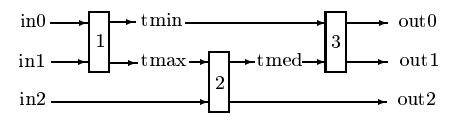
\includegraphics[width=\linewidth]{figures/sortingEx3.png}
		\caption{Mô tả về mạng sắp xếp với 3 phần tử \cite{altivec}}
		\label{fig:sortingEx3}
	\end{minipage}
	\hfill
	\begin{minipage}[b]{0.48\linewidth}
		\centering
		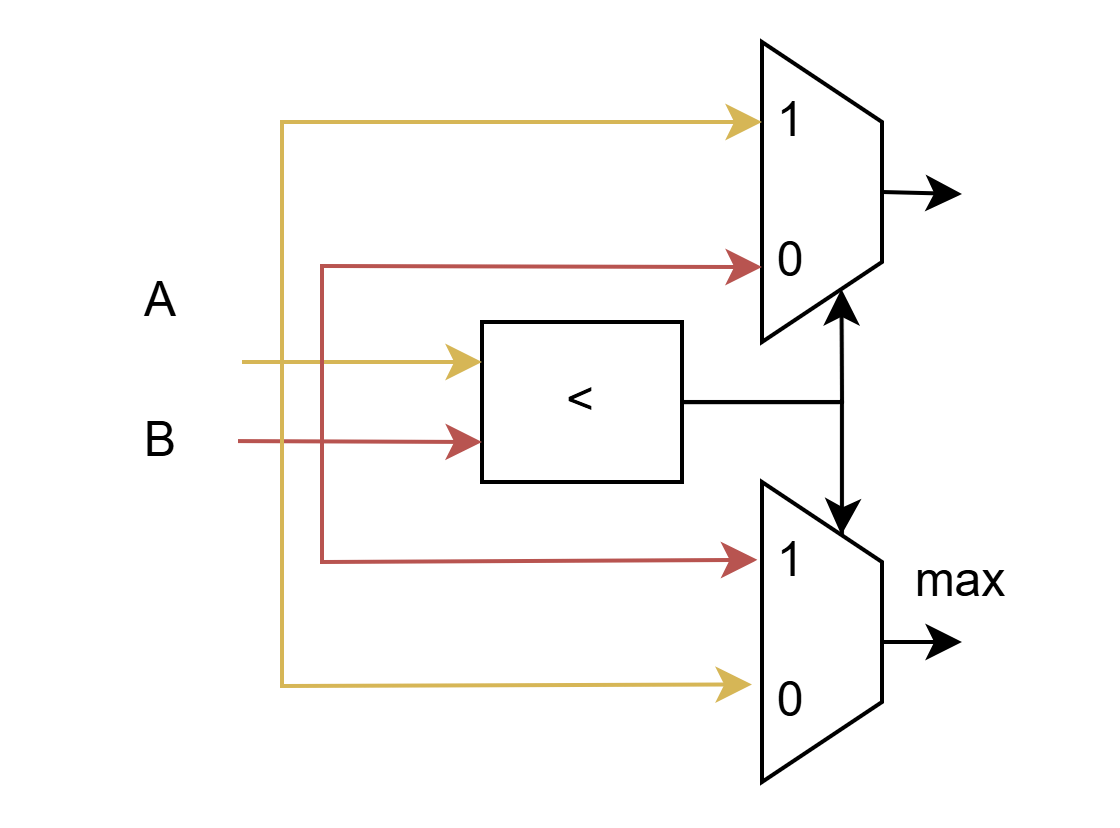
\includegraphics[width=\linewidth]{figures/node.png}
		\caption{Mô tả cấu trúc bộ so sánh và hoán đổi}
		\label{fig:node}
	\end{minipage}
\end{figure}
\subsubsection{Cửa sổ 3x3}

Hình \ref{fig:median3x3Exampel} mô tả nguyên lý và ví dụ về cách tìm giá trị trung vị của một ma trận kích thước 3x3. Với chuỗi đầu vào là 10, 9, 2, 5, 4, 3, 2, 2, 1. Giá trị trung vị ta mong đợi đạt được là 3. Các bước thực hiện bao gồm việc sắp xếp các hàng và các cột tăng dần. Sau khi đã xong hai bước trên, lúc này đường chéo gồm các phần tử 2, 4, 3. Lúc này, sẽ thực hiện sắp xếp theo thứ tự tăng dần, kết quả đạt được là 2, 3, 4. Vậy giá trị trung vị đạt được là 3, đã giống với giá trị mong đợi đạt được.  Hình \ref{fig:median3x3RTL} mô tả kiến trúc RTL của mô đun MedianCalculation với cửa sổ 3x3. Sinh viên đã thay thế các mạng sắp xếp khi đến bước sắp xếp cột để giảm độ tài nguyên phần cứng sử dụng (thay bộ Sorting\_network bằng chỉ 2 Node, vì không cần đủ 3 giá trị cho bước tiếp theo), hai là đã chèn thêm các thanh ghi giữa các bước để giảm trễ lan truyền, giúp tăng tần số hoạt động của mạch.
\begin{figure}[!ht]
	\centering
	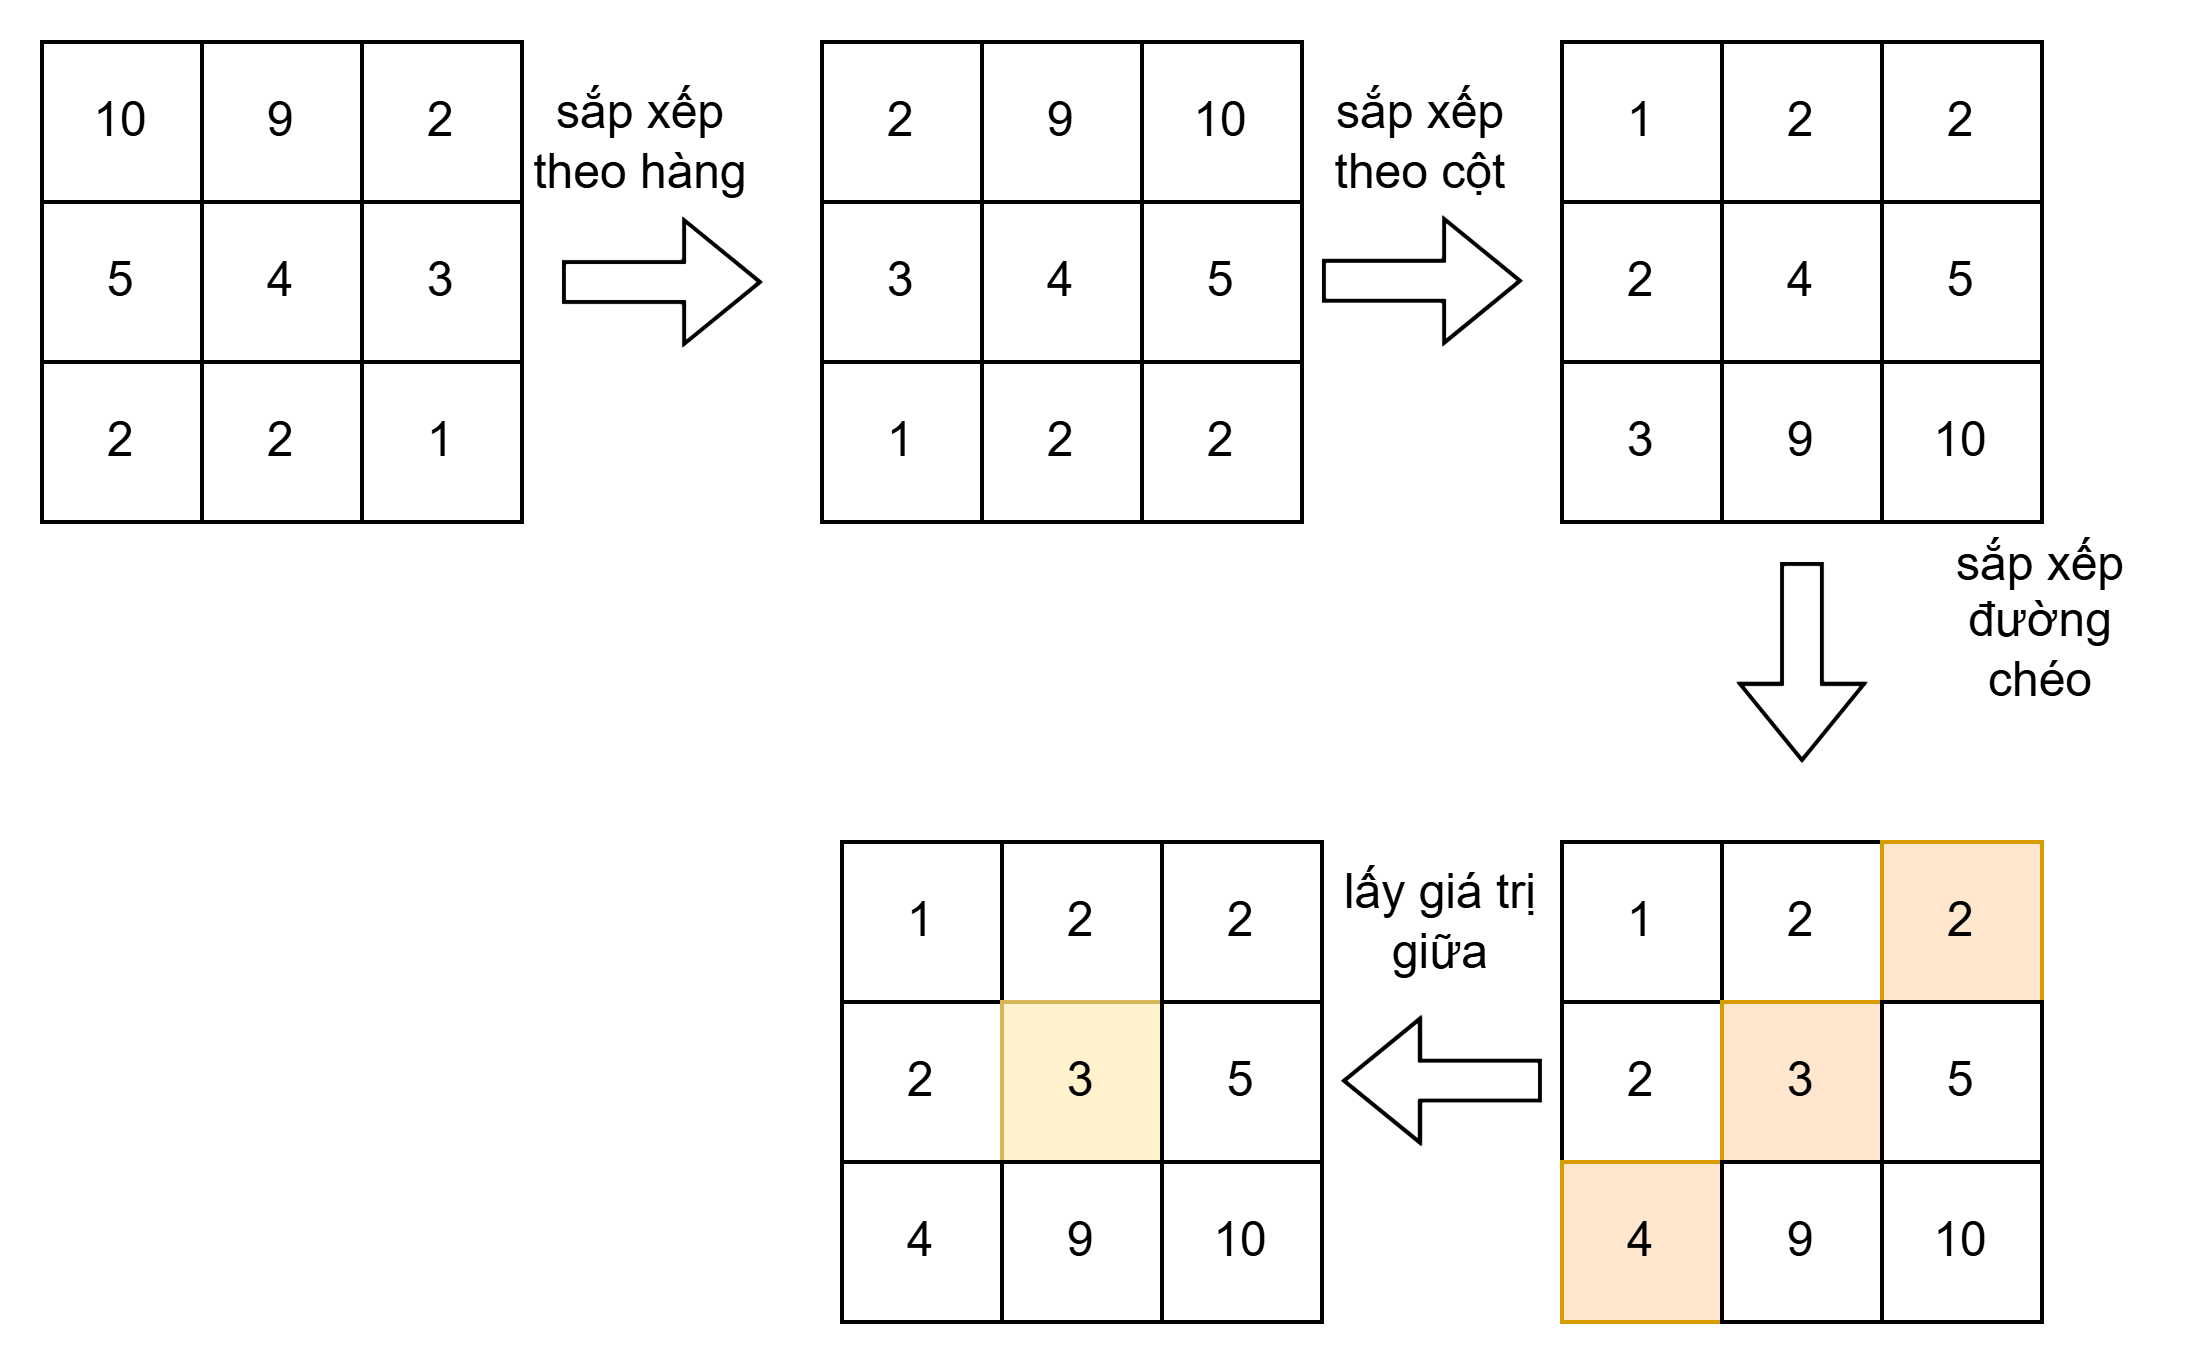
\includegraphics[width=0.6\linewidth]{figures/median3x3Exampel.png}
	\caption{Thực hiện và ví dụ của tìm trung vị của cửa sổ 3x3}
	\label{fig:median3x3Exampel}
\end{figure}
\begin{figure}[H]
	\centering
	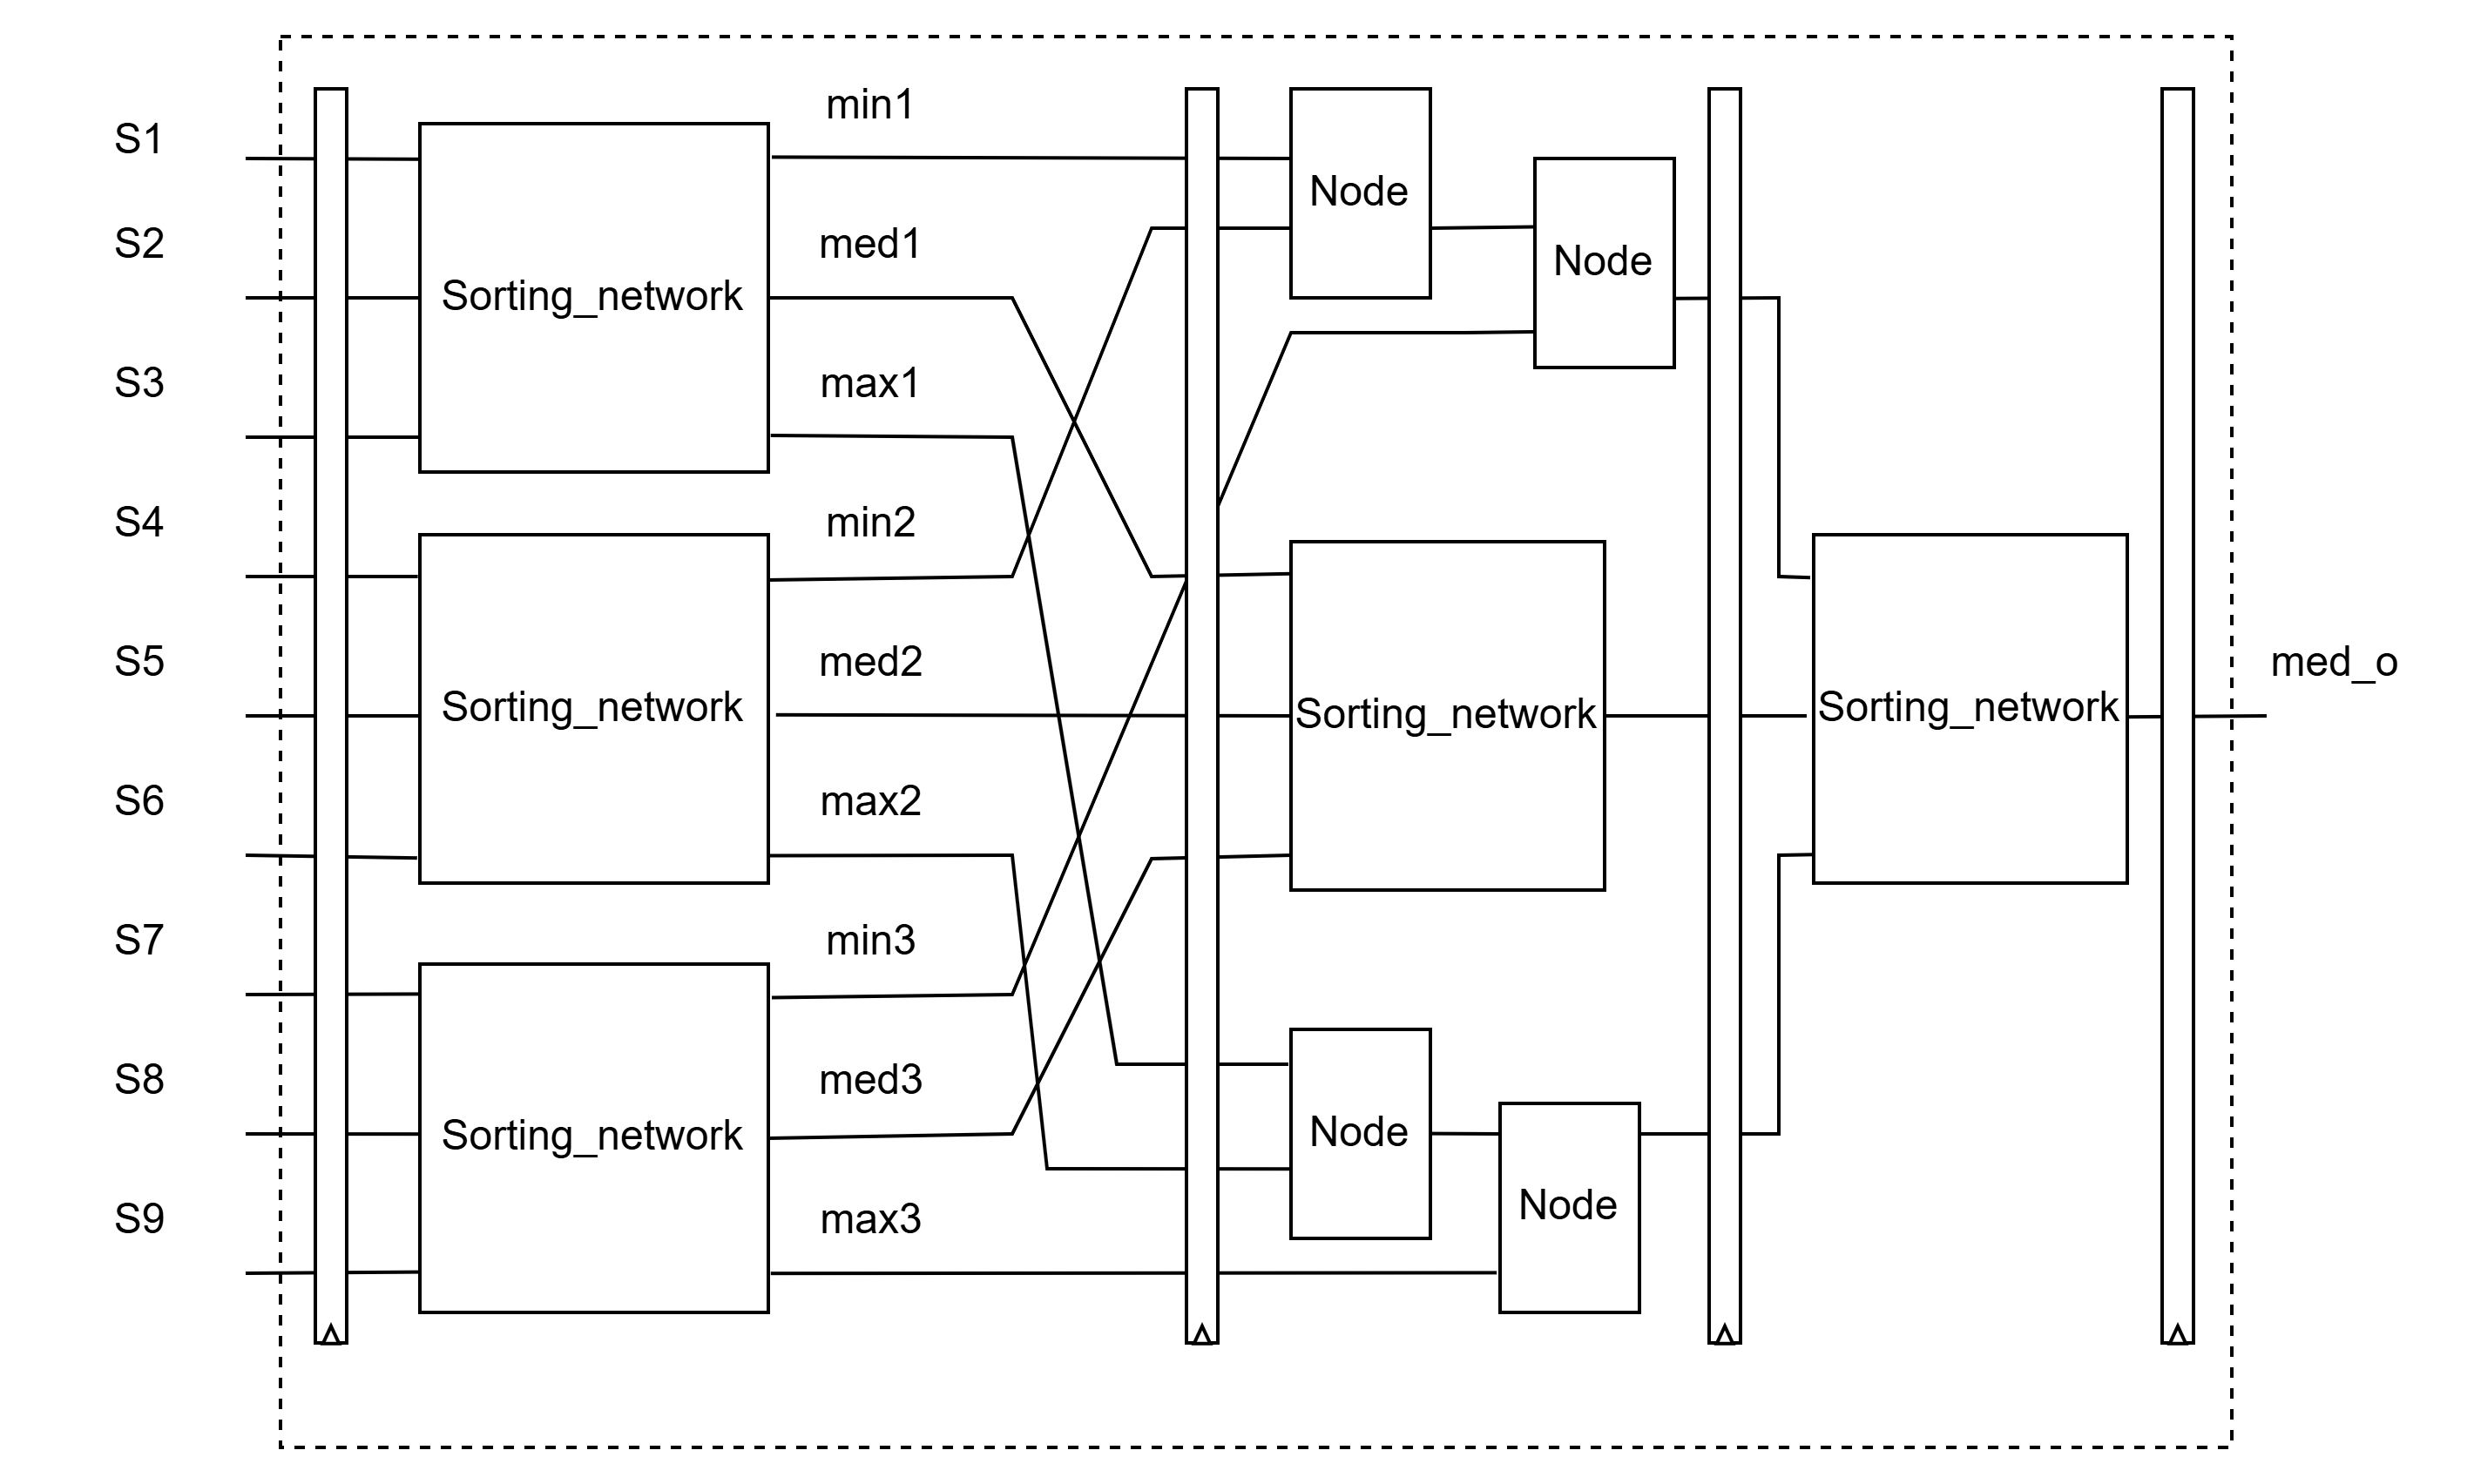
\includegraphics[width=\linewidth]{figures/median3x3RTL.png}
	\caption{Thực hiện và ví dụ của tìm trung vị của cửa sổ 3x3}
	\label{fig:median3x3RTL}
\end{figure}

\subsubsection{Cửa sổ 5x5}

Hình \ref{fig:median5x5Example} mô tả nguyên lý và ví dụ về cách tìm giá trị trung vị đối với cửa sổ 5x5. Để tối ưu cho tốc độ sắp xếp và sự không phụ thuộc, sinh viên sẽ thiết kế một sắp xếp 5 phần tử theo thứ tự tăng dần theo các bước được mô tả trong hình

\begin{figure}[!ht]
	\centering
	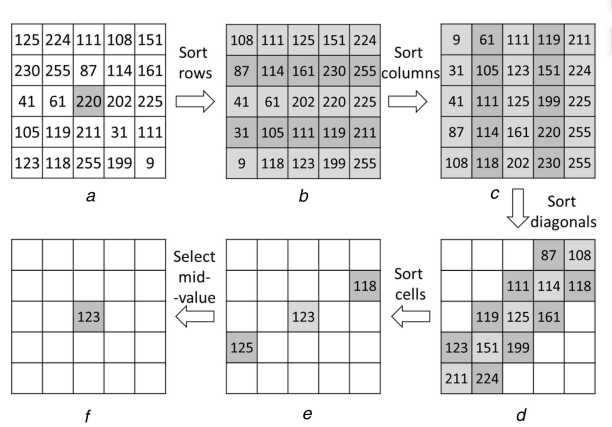
\includegraphics[width=0.8\linewidth]{figures/median5x5Example.png}
	\caption{Thực hiện và ví dụ của tìm trung vị của cửa sổ 5x5 \cite{llmf}}
	\label{fig:median5x5Example}
\end{figure}

\begin{figure}[!ht]
	\centering
	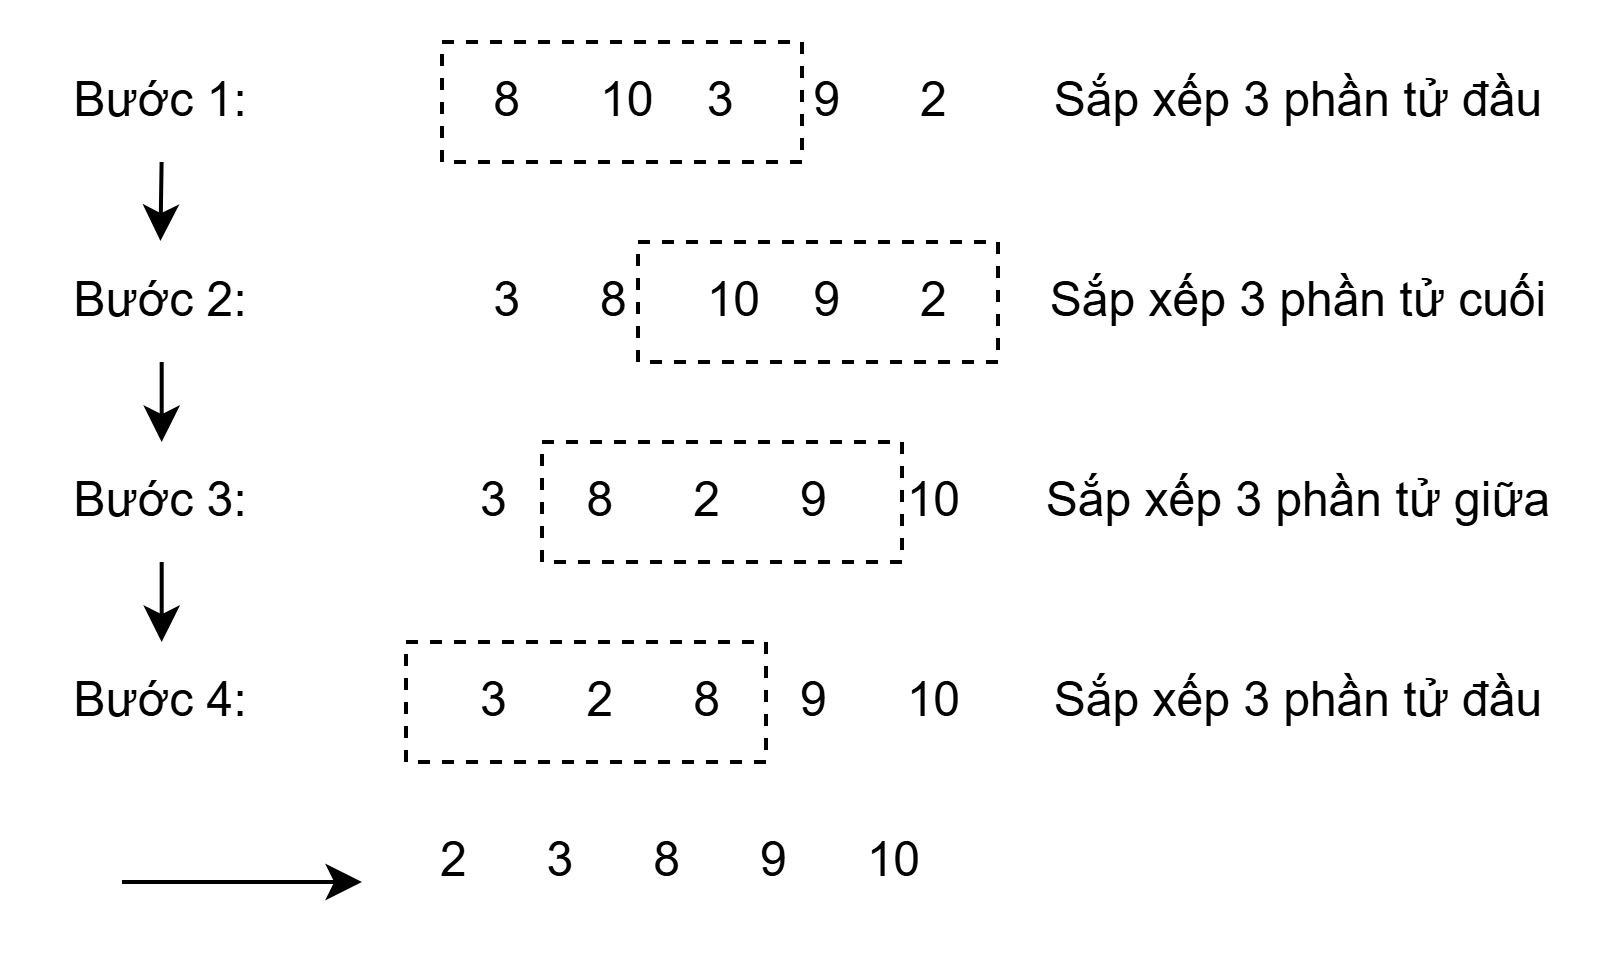
\includegraphics[width=0.8\linewidth]{figures/sortAscending5x5Ex.png}
	\caption{Xây dựng bộ sắp xếp 5 phần tử dựa trên bộ sắp xếp 3}
	\label{fig:sortAscending5x5Ex}
\end{figure}

\begin{figure}[!ht]
	\centering
	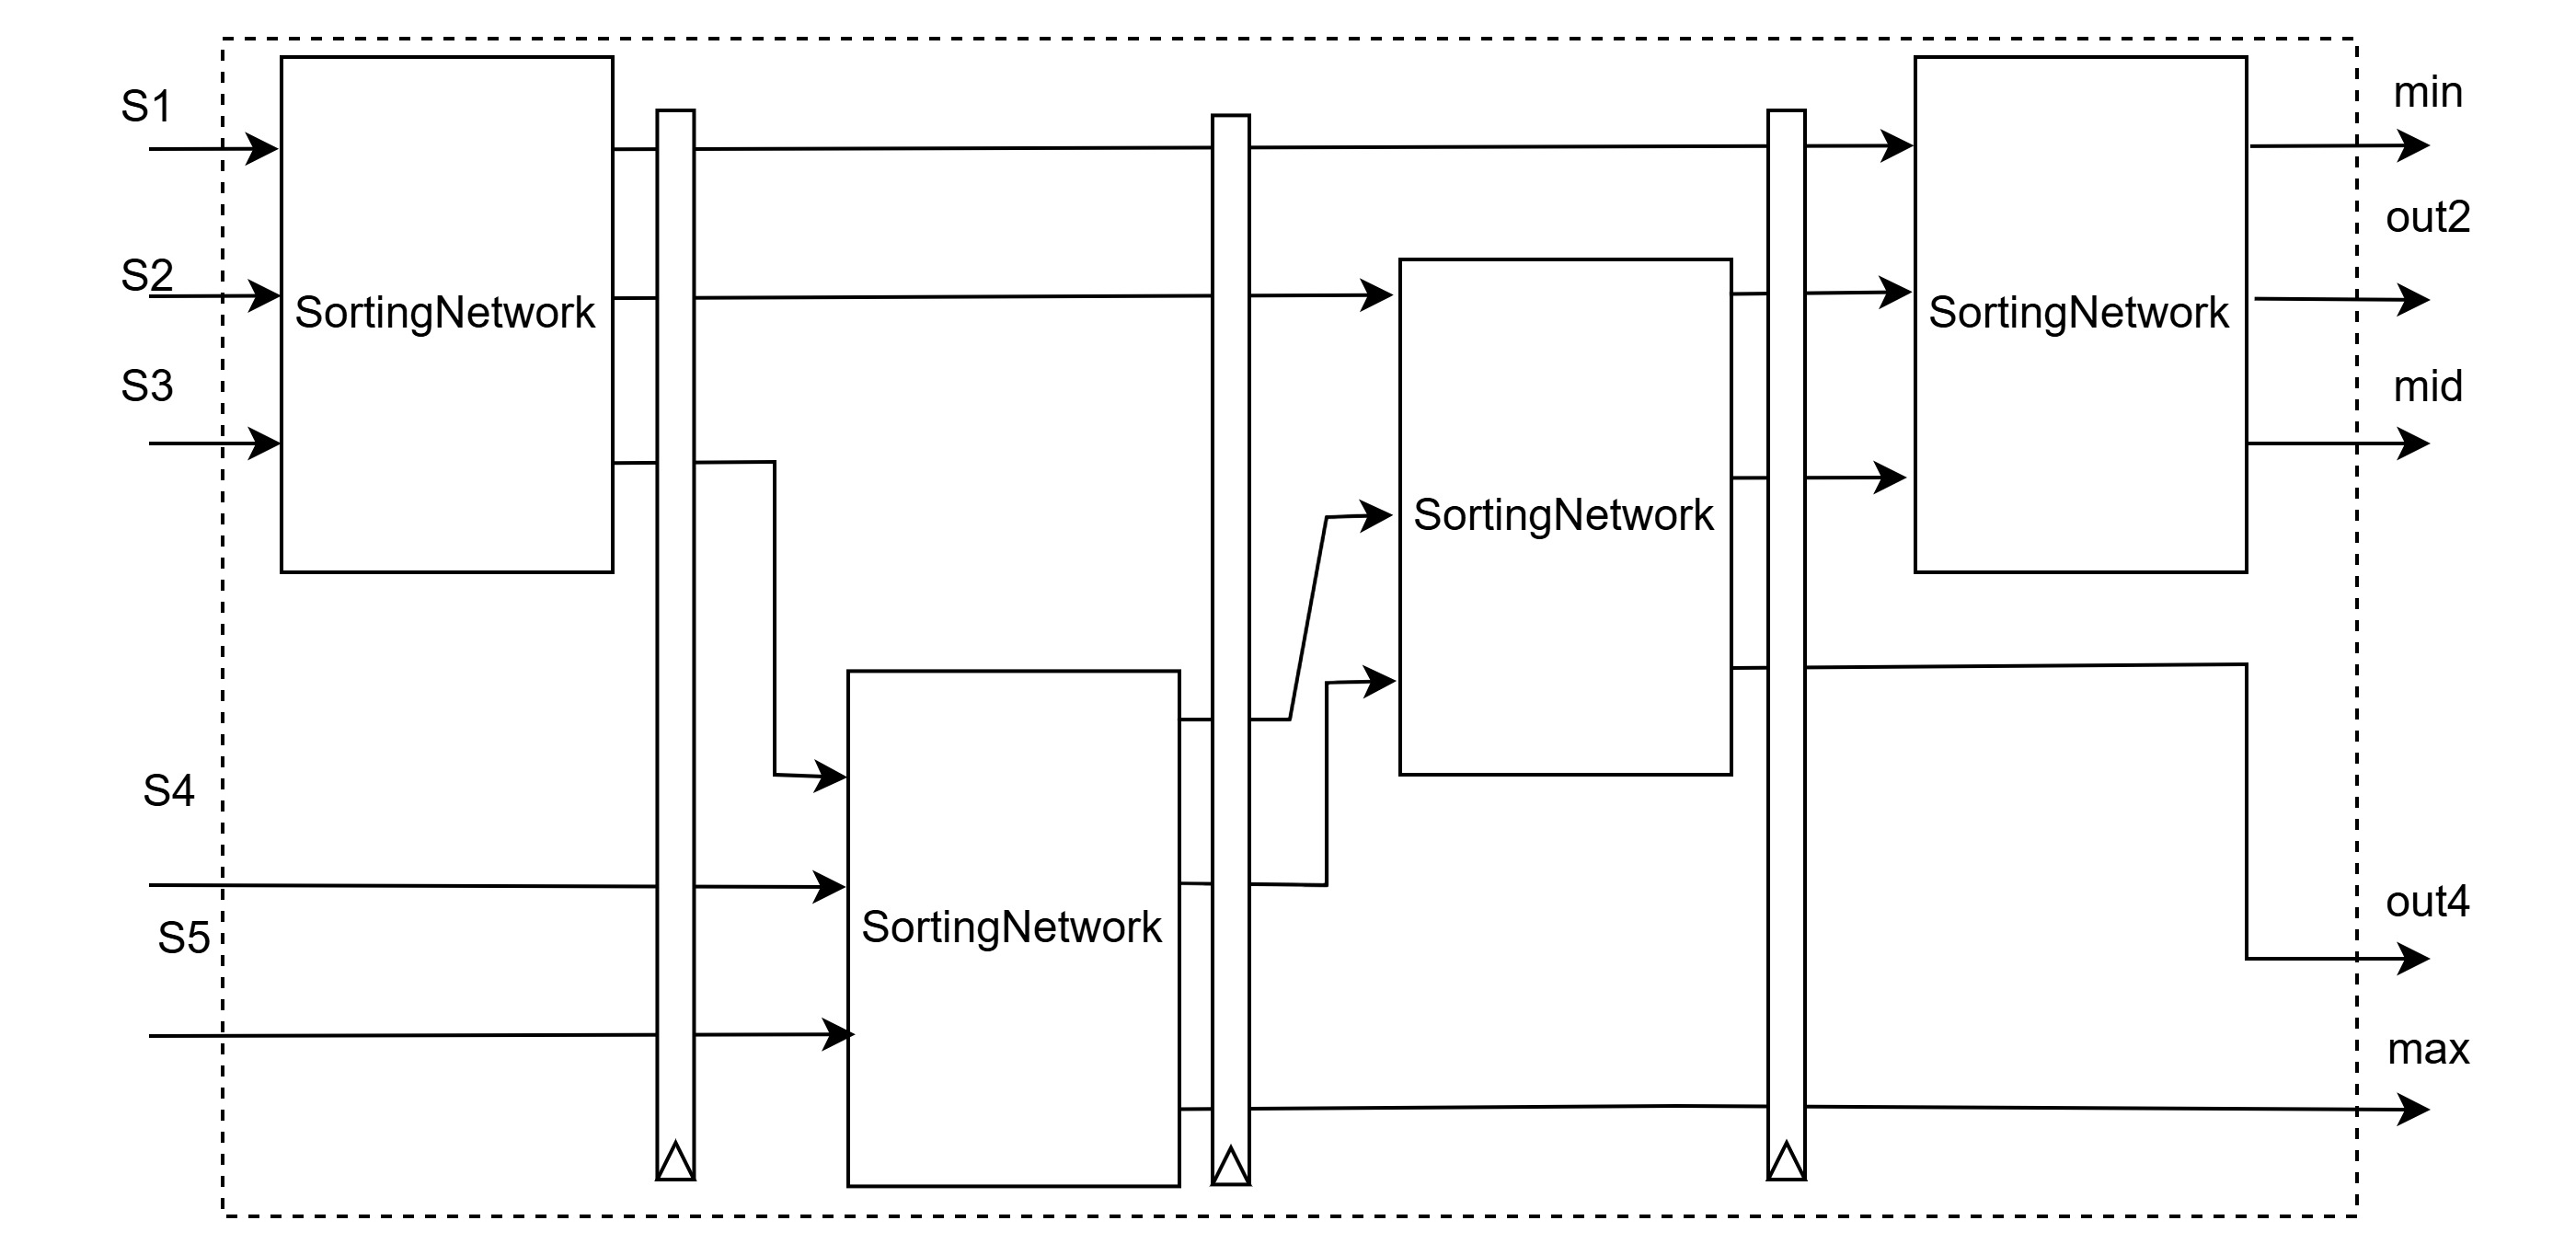
\includegraphics[width=\linewidth]{figures/sortAscending5x5RTL.png}
	\caption{Kiến trúc của bộ sắp xếp tăng dần 5 phần tử}
	\label{fig:sortAscending5x5RTL}
\end{figure}

\subsubsection{Cửa sổ 7x7}

Hình \ref{fig:median7x7Example} mô tả cách tìm ra giá trị trung vị đối với một ma trận kích thước 7x7. Điểm khác biệt đối với cửa sổ này là sau khi đã sắp xếp hàng và sắp xếp cột xong, ta sẽ tìm ra 25 phần tử thỏa mãn điều kiện, sau đó dựa vào bộ tìm trung vị đối với ma trận 5x5 để tìm trung vị chứ không thực hiện trực tiếp việc sắp xếp đường chéo theo mô tả tại thuật toán \ref{alg:medianFilterAlgo}. Sau khi sắp xếp theo hàng và cột xong, giá trị tại các ô xanh trong hình \ref{fig:median7x7Example} đã thỏa mãn điều kiện, tuy nhiên ở mỗi góc sẽ tồn tại 3 giá trị như mô tả tại ô màu vàng. Đối với phía trên, ta cần tìm giá trí lớn nhất của nó và đối với phía dưới, ta cần tìm giá trị nhỏ nhất. Từ đó, ta sẽ có đủ 25 phần tử và sử dụng nó có thể tìm kiếm được giá trị trung vị.

Để thực hiện sắp xếp tăng dần cho một cửa sổ 7x7, ta cần bộ sắp xếp tăng dần cho 7 phần tử, nó có thể được xây dựng trên các bộ sắp xếp 5 và bộ sắp xếp 3.
\begin{figure}[!ht]
	\centering
	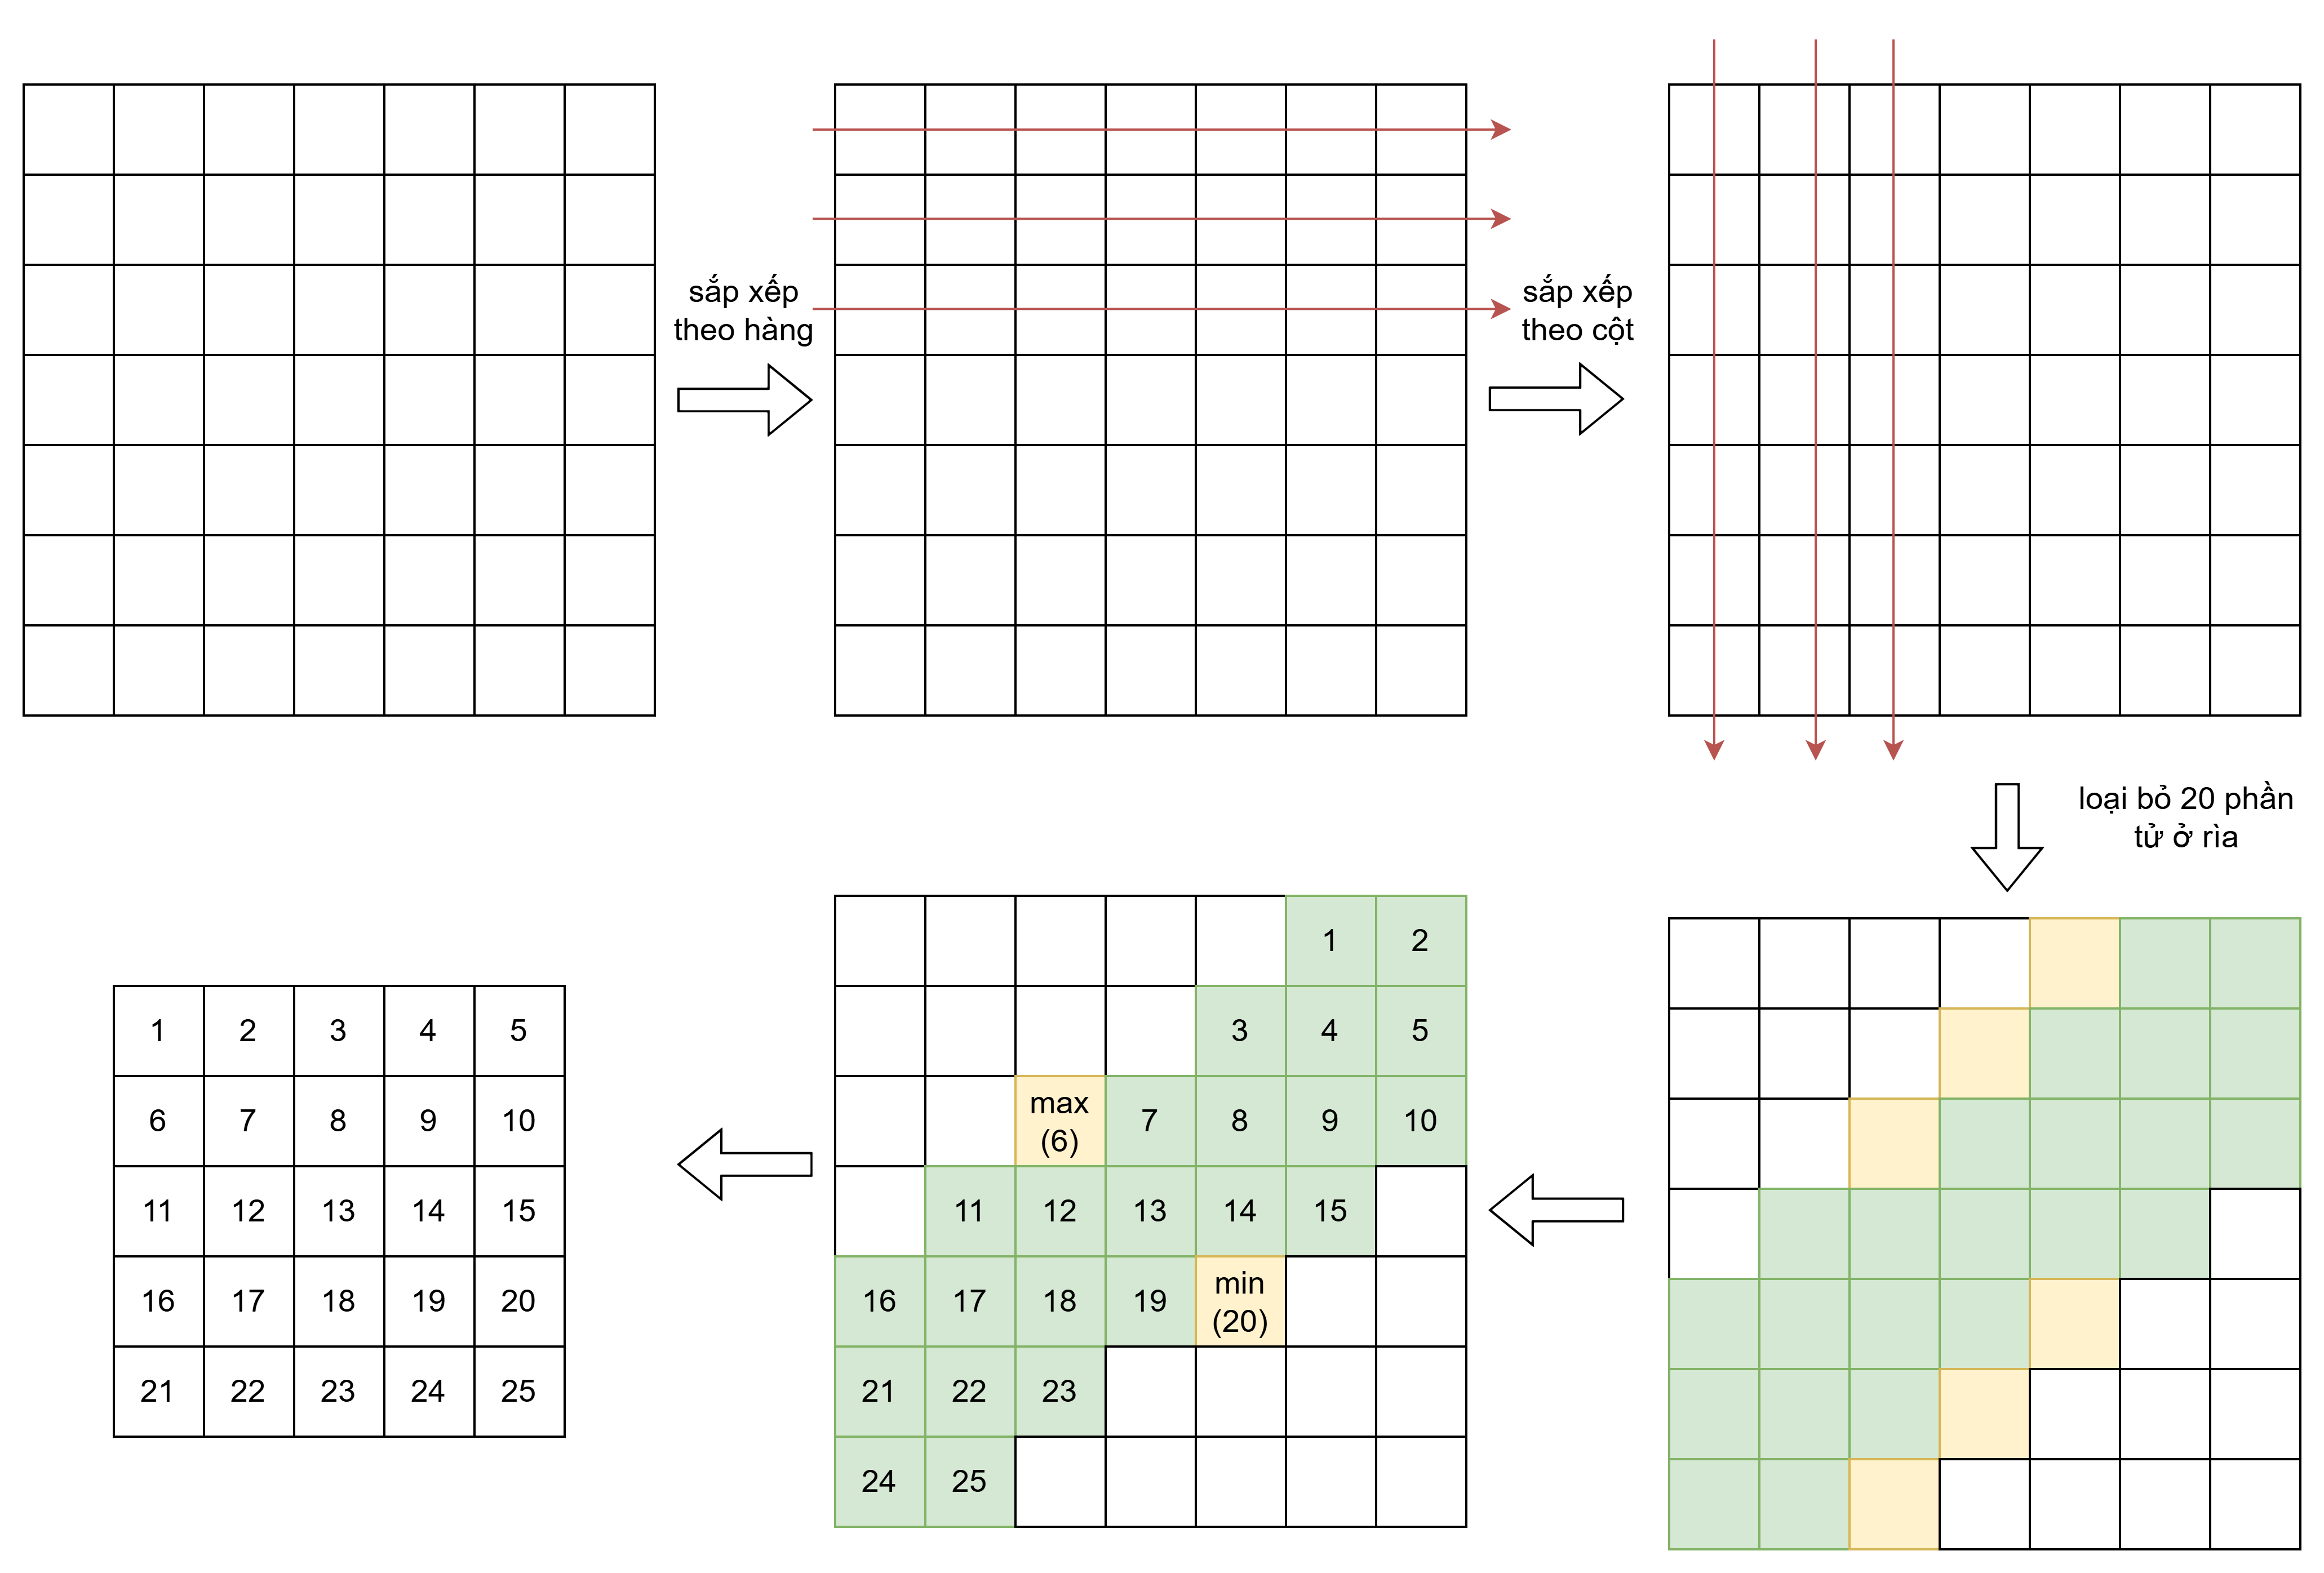
\includegraphics[width=\linewidth]{figures/median7x7Example.png}
	\caption{Thực hiện và ví dụ của tìm trung vị của cửa sổ 7x7}
	\label{fig:median7x7Example}
\end{figure}


